\documentclass[12pt, a4paper, oneside]{article}
\usepackage[utf8]{inputenc}
\usepackage[T1]{fontenc} % für besseres _ Zeichen
\usepackage[ngerman]{babel}
\usepackage{amsmath}
\usepackage{graphicx}
\usepackage{microtype} %besserer Randausgleich
\usepackage{footnote}
\usepackage{blindtext}
\usepackage{etoolbox}
\usepackage[pdfborderstyle={/S/U/W 1},hidelinks,breaklinks]{hyperref} % Für interaktive Refernzierung im PDF
\usepackage{csquotes}
\usepackage[acronym]{glossaries}
\usepackage[onehalfspacing]{setspace}%Zeilenabstand 1.5
\usepackage[ngerman]{babel}
\usepackage[top=2.5cm, bottom=2.5cm, left=2cm, right=3.5cm]{geometry}
\usepackage{bibgerm}
\usepackage{tabularx}
\usepackage{adjustbox}
\usepackage{blindtext}
\usepackage{epsfig}
\usepackage{float}
\usepackage{nameref}
\usepackage{bibentry}
\usepackage[backend=biber,style=alphabetic,sorting=ynt]{biblatex}
\usepackage{listings}
\usepackage{xcolor}
\usepackage{mathabx}
\usepackage{url}
%\usepackage[linesnumbered,lined,boxed,commentsnumbered]{algorithm2e}
\usepackage{caption}
\usepackage{subcaption}








\addbibresource{refs.bib}
\makeglossaries
\newglossaryentry{HODg}{
    name = {HOD},
	description = {Hands On Detection; ein System das einem Lenkrad ermöglicht 
        Griffe zu erkennen}, 
}

\newglossaryentry{SVNg}{
	name = {SVN},
	description = {Apache Subversion; eine freie Software zur zentralen 
        Versionsverwaltung von Dateien und Verzeichnissen}
}

\newglossaryentry{MVPg}{
	name = {MVP},
	description = {Minimal Viable Product (deutsch: minimal funktionsfähiges
        Produkt); Implementierung von lediglich den essenziellen Funktionen eines Produkts~\cite{Rie11}},
}

\newglossaryentry{Techniker}{
    name = {Techniker},
    description = {Eine Person, die Tests aufbaut und durchführt}
}

\newglossaryentry{Planer}{
    name = {Planer},
    description = {Eine Person, die die Durchführung der Tests plant}
}

\newglossaryentry{Backend}{
    name = {Backend},
    description = {Das in einer Server-Client-Architektur, auf dem Server 
        ausgeführte Programm}
}

\newglossaryentry{Frontend}{
    name = {Frontend},
    description = {Das in einer Server-Client-Architektur, auf dem Client 
        ausgeführte Programm, welches das \gls{UI} beinhaltet}
}

\newglossaryentry{Open-Source}{
    name = {Open-Source},
    description = {Software, deren Quellcode frei zugänglich ist und die 
        beliebig kopiert, genutzt und verändert werden darf~\cite{Dud22b}}
}

\newglossaryentry{APIg}{
    name = {API},
    description = {Eine Schnittstelle, die von verschiedenen Programmen benutzt 
        werden kann um die zur Verfügung gestellten Funktionen zu nutzen}
}

\newglossaryentry{RESTg}{
    name = {REST},
    description = {ein Paradigma für die Softwarearchitektur von verteilten 
        Systemen, insbesondere für Webservices}
}

\newglossaryentry{objektorientiert}{
    name = {objektorientiert},
    description = {ein Programmierparadigma, mit dem die Konsistenz von 
        Datenobjekten gesichert werden kann und das die Wiederverwendbarkeit
        von Quellcode verbessert~\cite{ErKa20}}
}

\newglossaryentry{Framework}{
    name = {Framework},
    description = {Programmiergerüst mit einsatzbereitem Code oder Softwareplattform~\cite{Dud22c}}
}

\newglossaryentry{dynamisch typisiert}{
    name = {dynamisch typisiert},
    description = {Datentypen einer dynamisch typisierten Programmiersprache
        können sich zur Laufzeit ändern}
}

\newglossaryentry{statisch typisiert}{
    name = {statisch typisiert},
    description = {Datentypen einer statisch typisierten Programmiersprache
        werden zur Kompilierzeit festgelegt und sind nicht änderbar}
}

\newglossaryentry{Garbage Collector}{
    name = {Garbage Collector},
    description = {eine automatische Speicherverwaltung}
}

\newglossaryentry{JSONg}{
    name = {JSON},
    description = {ein Datenformat zum Austausch von Daten zwischen Anwendungen}
}

\newglossaryentry{URIg}{
    name = {URI},
    description = {ein Identifikator, welcher zur Bezeichnung von Webseiten etc. verwendet wird (z.B. \textit{www.bht-berlin.de})}
}

\newglossaryentry{HTMLg}{
    name = {HTML},
    description = {eine Sprache zum strukturellen Aufbau eines elektronischen Dokuments (z.B. eine Webseite)}
}

\newglossaryentry{Jira}{
    name = {Jira},
    description = {Jira (entwickelt von Atlassian) ist eine Webanwendung zur Fehlerverwaltung, Problembehandlung und zum operativen Projektmanagement}
}

\newglossaryentry{JQLg}{
    name = {JQL},
    description = {eine Sprache zum filtern der Jira Datenbank}
}

\newglossaryentry{CSSg}{
    name = {CSS},
    description = {eine Formatierungssprache zur visuellen Bearbeitung von HTML Dokumenten}
}

\newglossaryentry{DOMg}{
    name = {DOM},
    description = {ein Interface um die Struktur, den Inhalt oder das Aussehen einer Webseite anzupassen}
}

\newglossaryentry{threadsicher}{
    name = {threadsicher},
    description = {eine Softwarekomponente, welche das gleichzeitige Bearbeiten durch mehrere Programmteile ermöglicht, ohne dass diese sich gegenseitig behindern, nennt man threadsicher}
}
\newglossaryentry{HOD}{
	type=\acronymtype,
	name = {HOD},
	description={Hands On Detection}, 
	first={Hands On Detection (HOD)\glsadd{HODg}},
	see=[Glossar:]{HODg}
}

\newglossaryentry{PDF}{
	type=\acronymtype,
	name = {PDF},
	description={Portable Document Format}, 
	first={Portable Document Format (PDF)},
}

\newglossaryentry{SVN}{
	type=\acronymtype,
	name = {SVN},
	description = {Apache Subversion},
	first={Apache Subversion (SVN)\glsadd{SVNg}},
	see=[Glossar:]{SVNg}
}

\newglossaryentry{JSS}{
	type=\acronymtype,
	name = {JSS},
	description = {Joyson Safety Systems},
	first={Joyson Safety Systems (JSS)},
}

\newglossaryentry{UI}{
	type=\acronymtype,
	name = {UI},
	description = {User Interface},
	first={User Interface (UI)}
}

\newglossaryentry{MVP}{
	type=\acronymtype,
	name = {MVP},
	description = {Minimal Viable Product},
	first={Minimal Viable Product (MVP)\glsadd{MVPg}},
	see=[Glossar:]{MVPg}
}

\newglossaryentry{API}{
	type=\acronymtype,
	name = {API},
	description = {Application Programming Interface},
	first={API\glsadd{APIg}},
	see=[Glossar:]{APIg}
}

\newglossaryentry{REST}{
	type=\acronymtype,
	name = {REST},
	description = {Representational State Transfer},
	first={REST\glsadd{RESTg}},
	see=[Glossar:]{RESTg}
}

\newglossaryentry{JSON}{
	type=\acronymtype,
	name = {JSON},
	description = {Javascript Object Notation},
	first={JSON\glsadd{JSONg}},
	see=[Glossar:]{JSONg}
}

\newglossaryentry{HTTP}{
	type=\acronymtype,
	name = {HTTP},
	description = {Hypertext Transfer Protocol},
	first={HTTP},
}

\newglossaryentry{URI}{
	type=\acronymtype,
	name = {URI},
	description = {Uniform Resource Identifier},
	first={Uniform Resource Identifier\glsadd{URIg}},
	see=[Glossar:]{URIg}
}

\newglossaryentry{HTML}{
	type=\acronymtype,
	name = {HTML},
	description = {Hypertext Markup Language},
	first={HTML\glsadd{HTMLg}},
	see=[Glossar:]{HTMLg}
}

\newglossaryentry{TCP}{
	type=\acronymtype,
	name = {TCP},
	description = {Transmission Control Protocol}
}

\newglossaryentry{ECU}{
	type=\acronymtype,
	name = {ECU},
	description = {Electronic Control Unit}
}

\newglossaryentry{JQL}{
	type=\acronymtype,
	name = {JQL},
	description = {Jira Query Language},
	first={JQL\glsadd{JQLg}},
	see=[Glossar:]{JQLg}
}

\newglossaryentry{CSS}{
	type=\acronymtype,
	name = {CSS},
	description = {Cascading Style Sheets},
	first={CSS\glsadd{JQLg}},
	see=[Glossar:]{JQLg}
}

\newglossaryentry{GUI}{
	type=\acronymtype,
	name = {GUI},
	description = {Graphical User Interface}
}

\newglossaryentry{DOM}{
	type=\acronymtype,
	name = {DOM},
	description = {Document Object Model},
	first={DOM\glsadd{DOMg}},
	see=[Glossar:]{DOMg}
}

\newglossaryentry{MVC}{
	type=\acronymtype,
	name = {MVC},
	description = {Model View Controller},
	first={Model-View-Controller}
}


\title{\textbf{Entwicklung einer Ressourcen-Übersicht auf Basis von Jira}}
\author{Nico Päller}

\setlength{\parindent}{0cm} %keine Einrückung
\linespread{1.5} 


\newpage
\newpage

\newcounter{SeitenzahlSpeicher}

\newcounter{desccount}
\newcommand{\descitem}[2]{%
  \item[\textbf{#1}] \refstepcounter{desccount}\label{#2}
}
\newcommand{\descref}[2]{\hyperref[#2]{\textbf{#1}}}
\newcommand{\descrefnobold}[2]{\hyperref[#2]{#1}}

\renewcommand{\lstlistingname}{Codebeispiel}% Listing -> Codebeispiel
\renewcommand{\lstlistlistingname}{Codebeispielverzeichnis}% 

\newcommand{\footurl}[1]{\footnote{\url{#1}}}


\newcolumntype{P}[1]{>{\centering\arraybackslash}p{#1}}

\begin{document}

\nocite{*}

\definecolor{codecomment}{rgb}{0.70, 0.70, 0.70}
\definecolor{codekeyword}{rgb}{0.83,0.14,0.44}
\definecolor{codestring}{rgb}{0.20,0.14,0.44}
\definecolor{backcolour}{rgb}{0.98, 0.98, 0.98}
\definecolor{jsonkey}{rgb}{0,0,0}

%% From https://tex.stackexchange.com/questions/195486/how-can-i-highlight-json-string-values-but-not-attributes
\newcommand\jsonkey{\color{jsonkey}}
\newcommand\jsonvalue{\color{codestring}}
\newcommand\jsonnumber{\color{codekeyword}}

% switch used as state variable
\makeatletter
\newif\ifisvalue@json

\lstdefinelanguage{json}{
    backgroundcolor=\color{backcolour},   
    commentstyle=\color{codecomment},
    keywordstyle=\color{codekeyword},
    numberstyle=\tiny\color{codecomment},
    stringstyle=\color{codestring},
    basicstyle=\ttfamily\footnotesize,
    breakatwhitespace=false,         
    breaklines=true,                 
    captionpos=b,                    
    keepspaces=true,                 
    numbers=left,                    
    numbersep=5pt,                  
    showspaces=false,                
    showstringspaces=false,
    showtabs=false,                  
    tabsize=4,
    keywords={false,true,null},
    alsoletter=0123456789,
    morestring          = [s]{"}{"},
    stringstyle         = \jsonkey\ifisvalue@json\jsonvalue\fi,
    MoreSelectCharTable = \lst@DefSaveDef{`:}\colon@json{\enterMode@json},
    MoreSelectCharTable = \lst@DefSaveDef{`,}\comma@json{\exitMode@json{\comma@json}},
    MoreSelectCharTable = \lst@DefSaveDef{`\{}\bracket@json{\exitMode@json{\bracket@json}}
}

\lstdefinelanguage{TypeScript}{
  keywords={typeof, new, true, false, catch, function, return, null, switch, var, if, in, while, do, else, case, break, let, const, then, JiraGroupedCCQueryResult},
  keywordstyle=\color{codekeyword}\bfseries,
  ndkeywords={class, export, boolean, throw, implements, import, this},
  ndkeywordstyle=\color{black}\bfseries,
  identifierstyle=\color{black},
  sensitive=false,
  comment=[l]{//},
  morecomment=[s]{/*}{*/},
  commentstyle=\color{codecomment}\ttfamily,
  stringstyle=\color{codestring}\ttfamily,
  morestring=[b]',
  morestring=[b]",
  morestring=[b]`,
  tabsize=2
}

% enter "value" mode after encountering a colon
\newcommand\enterMode@json{%
    \colon@json%
    \ifnum\lst@mode=\lst@Pmode%
        \global\isvalue@jsontrue%
    \fi
}

% leave "value" mode: either we hit a comma, or the value is a nested object
\newcommand\exitMode@json[1]{#1\global\isvalue@jsonfalse}

\lst@AddToHook{Output}{%
    \ifisvalue@json%
        \ifnum\lst@mode=\lst@Pmode%
            \def\lst@thestyle{\jsonnumber}%
        \fi
    \fi
    %override by keyword style if a keyword is detected!
    \lsthk@DetectKeywords% 
}

\makeatother

\lstdefinestyle{mystyle}{
    backgroundcolor=\color{backcolour},   
    commentstyle=\color{codecomment},
    keywordstyle=\color{codekeyword},
    numberstyle=\tiny\color{codecomment},
    stringstyle=\color{codestring},
    basicstyle=\ttfamily\footnotesize,
    breakatwhitespace=false,         
    breaklines=true,                 
    captionpos=b,                    
    keepspaces=true,                 
    numbers=left,                    
    numbersep=5pt,                  
    showspaces=false,                
    showstringspaces=false,
    showtabs=false,                  
    tabsize=2
}

\lstset{style=mystyle}


 \thispagestyle{empty}
\begin{titlepage}
	 \thispagestyle{empty}
	% thispagestyle{empty} unterdrückt Seitenzahlen auf der gewünschten Seite
	\newfont{\smc}{cmcsc10 at 12pt}
%	\maketitle
	%Aufpassen mit fi: Fehlercode U+FB01
	%%%%%%%%%%%%%%%%%%%%%%%%%%%%%%%%%%%%%%%%%%
%Titel, Autor, Seminar, Semester, Dozent %
%%%%%%%%%%%%%%%%%%%%%%%%%%%%%%%%%%%%%%%%%%
\begin{center}
	 \thispagestyle{empty}
\begin{figure}[t]
	\centering
	\includegraphics[width=0.8\textwidth]{./img/BHT_Logo_horizontal_Anthrazit_RGB_288ppi.png}
	
\end{figure}

$~~$\\
\textbf{\huge Entwicklung einer Resourcenübersicht auf Basis von Jira}\paragraph{}$~~$\\
\paragraph{}$~~$\\
\paragraph{}$~~$\\
\textbf{zwölfwöchige Abschlussarbeit im Rahmen der Prüfung}\\ \textbf{im Studiengang Elektromobilität (B.A.)}\\ \textbf{an der Berliner Hochschule für Technik}
\paragraph{}$~~$\\
\paragraph{}$~~$\\
\paragraph{}$~~$\\
\text{vorgelegt am: 14.04.2022}\\
\text{von: Nico Päller}\\
\text{Matrikelnummer: 892613}\\
\text{1. Gutachter: Prof. Dr. Sven Graupner}\\
\text{2. Gutachter: Alan Graf}\\
\paragraph{}$~~$\\
\text{Berliner Hochschule für Technik}\\
\end{center}	
\end{titlepage}



\pagenumbering{gobble}
\section*{Danksagung}
Diese Arbeit wäre ohne die Hilfe einiger Unterstützer nicht möglich gewesen.
Daher möchte ich mich bei Joyson Safety Systems für die Möglichkeit und die 
Unterstützung dieser Arbeit bedanken. Natürlich bedanke ich mich auch bei allen
Kollegen, mit denen ich Interviews durchführen durfte. Durch deren inhaltliche 
Anregungen konnte die Arbeit sich erst richtig entfalten. Ein besonderer Dank gilt
auch Ines Päller, die mir durch das gemeinsame Probelesen und gezielten Nachfragen 
zu besseren Formulierungen geholfen hat.

Zum Schluss möchte ich auch bei meinem Professor Graupner für die schnellen 
Rückmeldungen und gute Betreuung bedanken.

\newpage

Diese Arbeit verwendet das generische Maskulinum, um die Lesbarkeit zu erhalten.
Es sind dabei ausdrücklich alle Geschlechteridentitäten mitgemeint.

\newpage
\pagenumbering{arabic}

\begin{spacing}{1}
    \pagenumbering{Roman}
    \setcounter{page}{2}
    \tableofcontents
    \end{spacing}
    \newpage
    \begin{spacing}{1}
    \section*{Abbildungsverzeichnis} 
    \addcontentsline{toc}{section}{Abbildungsverzeichnis}
    \renewcommand{\listfigurename}{}
    \listoffigures
    \end{spacing}
    \newpage
    \section*{Tabellenverzeichnis} 
    \addcontentsline{toc}{section}{Tabellenverzeichnis} 
    \renewcommand{\listtablename}{}
    \listoftables % Tabellenverzeichnis
    \newpage
    % \section*{Symbolverzeichnis} 
    % \addcontentsline{toc}{section}{Symbolverzeichnis} 
    % %Sortieren nach Auftreten im Text
    % \begin{table}[h] \begin{center} \begin{tabular}{|lll|} \hline 
    % & \textbf{Symbol} & \textbf{Bedeutung} \\ \hline \hline
    % \end{tabular} \end{center} \end{table}
    % \newpage
    \addcontentsline{toc}{section}{Akronyme}
    \printglossary[type=\acronymtype]
    \newpage
    \addcontentsline{toc}{section}{Glossar}
    \printglossary[type=main]
    \newpage
    \lstlistoflistings
    \newpage
    \clearpage
    \setcounter{SeitenzahlSpeicher}{\value{page}}
    \pagenumbering{arabic}
    \newpage
    \pagenumbering{arabic}

\section{Einführung}

Die Effizienz in einem Unternehmen spielte schon immer mehr eine wichtige Rolle,
da es häufig viele Deadlines gibt, die eingehalten werden müssen. Effizientes 
Arbeiten benötigt jedoch nicht nur eine genaue Planung, sondern auch eine 
Möglichkeit für alle Beteiligten, die vorgesehenen Prozessschritte einzusehen 
und einzuhalten. Gerade im Bereich der Digitalisierung, gibt es viel Potential, 
Prozesse effizienter zu gestalten. Circa ein Drittel der Maschinenbau- und 
Anlagenbau Unternehmen sehen eine Effizienzsteigerung durch die 
Digitalisierung~\cite{Bre17}. So können Prozesse teilweise oder voll automatisiert
werden, um die Arbeitszeiten und den Arbeitsaufwand von Mitarbeitern und Mitarbeiterinnen
auf ein minimum zu beschränken. 

\subsection{Problemstellung}\label{sec:problems}
Bei Joyson Safety Systems in der Abteilung ``\gls{HOD} System Test'' werden die 
durchzuführenden Tests mittels der Ticketsoftware \gls{Jira} geplant. Jeder durchzuführende
Test erhält dabei pro Muster ein eigenes Ticket. Eine ganze Testreihe 
beinhaltet meistens hunderte einzelne Tests, welche in einer gewissen
Reihenfolge durchgeführt werden müssen. 

Nachdem eine Testreihe einplant wurde, wird jeden Morgen ein Tagesplan 
erstellt, in welchem genau beschrieben ist, welcher Test auf welche Weise 
durchzuführen ist. Dieser Plan liegt als Auszug eines \gls{Jira} Filters inf Form 
einer statischen HTML Datei vor (Siehe Abb.~\ref{fig:tagesplan}). Dadurch sind 
die Informationen, welche die \gls{Techniker} erhalten auf das Wichtigste begrenzt. 

Um die Zeit des Umbaus zu minimieren und die verfügbare Zeit einer Klimakammer
für Tests zu maximieren, muss ein \gls{Techniker} jedoch wissen, was er für den 
nächsten Test umbauen muss. Diese Information steht ausschließlich im \gls{Jira}  
Ticket zur Verfügung, weshalb das Nachsehen im Ticket für jeden Test einen
erheblichen Aufwand darstellt.

\begin{figure}[H]
    \includegraphics[width=\linewidth]{img/jira-ticket.png}
    \caption{\gls{Jira} Ticket}
\end{figure}

Solch ein \gls{Jira} Ticket ist zu unübersichtlich, um schnell alle wichtigen 
Informationen zu erhalten. Wichtige Daten, wie etwa das zu verwendende Zubehör
sind nur in unstrukturierter Form in den Labels des Tickets vorhanden. 
Außerdem bringt das Heraussuchen jedes Tickets einen gewissen Zeitaufwand mit sich.\\

Ein weiteres Problem ist, dass die Wartungsinformationen momentan lediglich in einer Excel
Tabelle gespeichert und vom Wartungsbeauftragten gepflegt werden. Somit
wissen der \gls{Techniker} oder der \gls{Planer} nicht genau, ob das geplante 
Zubehör auch wirklich verwendet werden darf. Er muss sich folglich darauf verlassen, 
dass es rechtzeitig gewartet wurde, da ein Nachsehen in der Liste einen zu hohen
Aufwand bedeuten würde.\\

\newpage
Aus den zuvor genannten Situationen treten folgende Probleme hervor:

\begin{description}

    \item[1. Heraussuchen der Jiratickets für Informationen]\hfill \\
    Wenn der Techniker beispielsweise beim Umbau eines Tests wissen möchte,
    welcher Test folgt, muss er sich in \gls{Jira} anmelden. Danach muss er das Ticket über die
    Testrun-ID aus dem Tagesplan suchen und im Ticket einsehen, ob der nächste 
    Test verlinkt ist. Da in einer Klimakammer meistens 3 Muster getestet werden,
    muss dieser Prozess für jedes weitere Muster wiederholt werden. Das ist ein 
    zu hoher zusätzlich zum Umbau hinzukommender Zeitaufwand. Denn um den maximalen
    betriebswirtschaftlichen Nutzen der Klimakammern zu ermöglichen, muss die 
    Umbauzeit so gering wie möglich gehalten werden.
    

    \item[2. Wartungsdatum eines Zubehörs einsehen und anpassen]\hfill \\
    Wenn ein Mitarbeiter wissen möchte, wann ein gewisses Zubehör gewartet werden muss oder ob 
    es verwendet werden darf, muss er in einer Excel Datei nach dem entsprechenden
    Zubehör suchen. Da diese Excel Datei im \gls{SVN} abgelegt ist, wird sie auch nur
    darüber mit allen weiteren Benutzern synchronisiert. Dabei kann es auch zu 
    unterschiedlichen Versionen der Datei kommen, wenn beispielsweise ein Mitarbeiter 
    vor dem Einsehen der Datei seine \gls{Working Copy} nicht aktualisiert.

    \item[3. Universelle Schnittstelle]\hfill \\
    Es ist zudem notwendig, gerade die Wartungsdaten schon beim Vorbereiten der Tests
    zugänglich zu machen. Somit kann der \gls{Techniker} schon vor dem Umbau wissen,
    ob alle im nächsten Test verwendeten Ressourcen auch tatsächlich für die 
    Verwendung geeignet sind.
    Auf Grundlage dieser Informationen, kann er die nötigen Ressourcen vorbereiten, sodass der
    Zeitaufwand des Umbaus minimiert wird.
    Da für die Vorbereitung jedoch ein separates Programm verwendet wird, müssen
    die von dieser Arbeit bereitgestellten Informationen universell von Programmen
    und Entwicklern abrufbar sein.
\end{description}

\newpage

\subsection{Zielsetzung}
Das Programm wird unter dem Namen ``TestHub'' innerhalb der Firma \gls{JSS} 
veröffentlicht. Die Arbeit hat folgende Ziele:

\begin{itemize}
\item Entwicklung einer interaktiven Übersicht zum schnellen Überblick über Wartungstermine, aktuelle, vorherige und folgende Tests 
\item Aufbereitung und Kategorisierung der Daten in den Labels eines \gls{Jira} Tickets
\item Zentrale Speicherung, Einsicht und Anpassung von Testzubehörinformationen
\item Entwicklung einer universell erreichbaren Schnittstelle, zur Integration der von dieser Arbeit bereitgestellten Informationen in andere Softwareprojekte

\end{itemize}

Die Entwicklung von TestHub lässt sich in zwei grobe Punkte unterteilen:

\begin{description}

    \item[1. Entwicklung des Backends]\hfill \\
    Das Backend ist die zentrale serverseitige Software, welche die nötigen 
    Daten von \gls{Jira} oder einer Datenbank sammelt und anschließend in standardisierten Formaten über das Internet 
    versendet.
    

    \item[2. Entwicklung des UI]\hfill \\
    Um die Daten visuell und kompakt darzustellen, gibt es ein Interface, 
    welches die vom Backend empfangenen Daten übersichtlich auf einer Webseite
    anzeigt

\end{description}


Durch eine Trennung des \gls{Backend}s und des \gls{Frontend}s entstehen verschiedene 
Vorteile. Zum einen können andere Programme das Backend ebenfalls benutzen und
die nötigen Daten bei sich integrieren. Es lässt sich außerdem leicht erweitern.
Zum anderen lässt sich das \gls{UI} leicht austauschen bzw. anpassen, da es lediglich 
die vorhandenen Daten anzeigt. \\

Testhub ist als \gls{MVP} entwickelt. Es werden daher nur die wichtigsten in 
Abschnitt~\ref{sec:fas} und Abschnitt~\ref{sec:nfas} genannten Anforderungen implementiert.


\subsection{Vorgehensweise}
Die vorliegende Arbeit wird in mehrere Kapitel unterteilt:

\begin{description}

    \item[Kapitel 1: Einleitung:]
    In der Einleitung werden die Problemstellung und die Ziele inklusive der Motivation
    dieser Arbeit beschrieben.
    
    \item[Kapitel 2: Grundlagen:]
    Im Kapitel über die Grundlagen werden Implementierungsmöglichkeiten diskutiert
    und abgewogen. Zusätzlich wird dort kurz die Abteilung und das zentrale Glied
    dieser Arbeit, die \gls{REST} \gls{API} erklärt.

    \item[Kapitel 3: Anforderungsanalyse:]
    Eine Analyse der aktuellen Prozesse findet in Kapitel 3 statt. Darauf basierend werden Anforderungen an 
    das zu entwickelnde Programm definiert.

    \item[Kapitel 4: Entwurf:]
    Im Entwurf wird sowohl die Softwarearchitektur des Programms als auch die Gestaltung 
    des \gls{UI} beschrieben.
    
    \item[Kapitel 5: Entwicklung:]
    Der Entwicklungsteil der Arbeit erläutert sowohl die Implementierung als auch 
    den Softwarelebenszyklus des gesamten Projekts.

    \item[Kapitel 6: Validierung:]
    Die in Kapitel 3 ermittelten Anforderungen werden in diesem Kapitel den
    tatsächlichen Funktionen des Programms gegenübergestellt und verifiziert.

    \item[Kapitel 7: Fazit:]
    Das letzte Kapitel fasst die Ergebnisse dieser Arbeit zusammen. Zusätzlich werden die
    die nächsten Schritte der Weiterentwicklung besprochen.

\end{description}
\newpage





\section{Grundlagen}
In diesem Kapitel werden die Grundlagen der im \gls{HOD} System Test erläutert.
Anschließend wird auf das zentrale Element der Arbeit, die REST API eingegangen.
Zusätzlich werden Programmiersprachen zur Entwicklung vom \gls{Backend} 
gegenübergestellt und eine potenzielle Verwendung abgewogen.

\subsection{HOD Systemtest}
Die Abteilung Hands-On-Detection entwickelt ein Lenkrad, welches durch eine 
kapazitive Matte im Lenkrad erkennen kann, ob und wie ein Lenkrad berührt wurde.
Dieses System muss nicht nur entwickelt sondern auch ausgiebig getestet werden.
Da Joyson nach dem V-Modell testet, werden die Tests auf mehrere Ebenen verteilt.
Die Ebene des Systemtests, testet das ganze System, das heißt es wird das ganze
Lenkrad mit der von Joyson entwickelten \gls{ECU} getestet.

\begin{figure}[H]
    \includegraphics[width=8cm,keepaspectratio]{img/duts_in_cc.jpg}
    \centering
    \caption{HOD Lenkräder in einer Klimakammer}
\end{figure}

Die verschiedenen Funktionen der Lenkräder wird bei -40°C bis 80°C getestet. 
Dabei werden meistens 3 Lenkräder in einer Klimakammer getestet. Alle, für 
diese Tests verwendeten Teile, wie Kabelbäume, Messhardware, die Klimakammer etc.,
werden Ressourcen genannt.


\subsection{REST API}\label{sec:restapi}
Seit der ersten Website von Tim Berners-Lee 1991 wächst das Web teilweise 
exponentiell. Allerdings war das Web nicht für solch ein rasantes Wachstum gemacht.
Es gab weder einheitliche Kommunikationsprotokolle, noch konnte die Infrastruktur
den Datenverkehr standhalten. Alarmiert von diesem Problem, entwickelte Roy Fielding
eine Web Architektur, welche die Bedingungen des Webs einheitlich lösen soll.
Diese Bedingungen lassen sich in 6 Kategorien zusammenfassen~\cite{Mas11}:

\begin{description}

    \item[1. Client-Server]\hfill \\
    Die Client-Server Struktur stellt eine Trennung der Anliegen dar. Der Client
    fordert dabei einen Dienst oder eine Information an, welche der Server erfüllt.
    Die Technologie welche zum Entwickeln von Client und Server verwendet wird,
    spielt dabei keine Rolle, solange sie das einheitliche Interface implementieren.

    \item[2. Einheitliches Interface]\hfill \\
    Mark Massé fasst in seinem Buch \textit{Rest Api: Design Rulebook}~\cite{Mas11}
    das einheitliche Interface in 4 Anforderungen zusammen: 
    
    \begin{enumerate}
        \item Identifikation von Ressourcen\hfill \\
        Jedes webbasierte Konzept (Ressource) muss über einen einzigartigen 
        \gls{URI} adressiert werden können. 

        \item Manipulation von Ressourcen durch Repräsentationen\hfill \\
        Clients müssen die Ressourcen manipulieren können, indem Sie mit verschiedenen
        Repräsentationen arbeiten. Beispielsweise kann ein Dokument sowohl in 
        \gls{JSON} für ein automatisiertes Programm als auch als \gls{HTML} für 
        einen Webbrowser repräsentiert werden. Dadurch lässt sich laut Massé eine
        Interaktion mit dem Dokument gewährleisten, ohne das Dokument und seinen
        Identifier zu verändern.

        \item Selbstbeschreibende Nachrichten\hfill \\
        Wenn der Client eine Anfrage schickt, ist dies nur der gewünschte Zustand
        der Ressource. Der tatsächlich aktuelle Zustand, ist repräsentativ in 
        der Antwort des Servers enthalten. Wenn also jemand einen Kommentar bei 
        YouTube schreibt, schlägt er nur den Inhalt des Kommentars vor. Ob der 
        Kommentar tatsächlich übernommen und angezeigt wird, hängt allein vom 
        Server ab. 
        Um diese selbstbeschreibenden Nachrichten mehr Informationen über die 
        versendete oder angefragte Ressource enthalten zu lassen, können Metadaten
        in den Nachrichten enthalten sein. Diese Metadaten können zum Beispiel
        die Art der Repräsentation, die Länge der Daten oder eine Authentifizierung 
        sein.\\

        Bei einer \gls{HTTP}-Nachricht werden diese Metadaten in die ``Header'' 
        geschrieben, welche vordefinierte Zwecke besitzen.

        \item Hypermedien als Antrieb des Applikationsstatuses\hfill \\
        Laut Massé, sind Links die ``Fäden die das Netz zusammennähen''~\cite[][4]{Mas11}.
        Daher sollte es in dem einheitlichen Interface die Möglichkeit eine Navigation
        der Informationen durch Links geben.

    \end{enumerate}

    \item[3. Schichtsystem]\hfill \\
    Durch ein Schichtsystem soll ermöglicht werden, Zwischensysteme, wie einen
    Proxy Server oder ein Gateway zu etablieren. Diese Systeme werden benötigt, 
    um beispielsweise Sicherheitsstandards zu erzwingen oder um viele gleichzeitige
    Anfragen auf die vorhandene Hardware zu balancieren (load balancing).

    \item[4. Caching]\hfill \\
    Caching ist das Zwischenspeichern von Informationen. Um den Server zu entlasten
    und somit Geld zu sparen und zusätzlich die Latenz des Clients zu verringern,
    sollten Ressourcen zwischengespeichert werden, sodass bei einer erneuten 
    Anfrage die zwischengespeicherte Version geladen wird und keine neue 
    Datenübertragung initialisiert werden muss. Caching wird von allen modernen 
    Webbrowsern automatisch betrieben, kann aber auch von den oben genannten
    Zwischensystemen umgesetzt werden.

    \item[5. Zustandslosigkeit]\hfill \\
    Die Anforderungen der Zustandslosigkeit beschreibt, dass alle kontextuellen 
    Informationen in der Anfrage des Clients enthalten sein muss, sodass der 
    Server keine Informationen zum Client speichern muss. Dadurch kann der Server
    wesentlich mehr Anfragen bearbeiten, das der Aufwand pro Anfrage gering 
    gehalten wird. Die Zustandslosigkeit trägt erheblich zur Skalierung der
    Architektur des Webs bei, laut Massé~\cite[][4]{Mas11}. 

    \item[6. Code-On-Demand]\hfill \\
    Code-On-Demand ist die Möglichkeit, ausführbare Skripte oder Programme vom 
    Server an den Client zu schicken. Da der Client jedoch den empfangenen Code
    verstehen und ausführen muss, ist dies die einzige optionale Anforderung an
    die Architektur des Webs.
\end{description}

Diese zuvor genannten Anforderungen, werden elegant durch eine \gls{REST} \gls{API}
erfüllt. REST steht für Representational State Transfer und beschreibt eine Ansammlung von
Regeln, nach welchem man seine \gls{API} architektonisch aufbauen sollte. Diese 
Regeln lassen sich jedoch auf die unterschiedlichsten Weisen implementieren. 

\subsection{HTTP Kommunikation}\label{sec:HTTP}
Das Hypertext Transfer Protokoll (kurz HTTP) regelt die Datenübertragung zwischen
Anwendungen. Viele \gls{REST} \gls{API}s verwenden HTTP, da dieses gewisse
Anforderung, wie die Zustandslosigkeit, bereits implementiert. Im Folgenden soll
die Funktionsweise vom HTTP erläutert werden, da dies grundlegend für sowohl ``TestHub''
als auch die \gls{JIRA} Kommunikation ist.

\subsubsection{Allgemeines}
HTTP implementiert verschiedene Anfragetypen und Headertypen. Die wichtigsten,
welche auch von der \gls{REST} \gls{API} von ``TestHub'' verwendet wird, werden 
hier aufgelistet:

\begin{table}[h!]
    \centering
    \begin{tabular}{|c | c|} 
     \hline
     \textbf{Anfragetyp} & \textbf{Beschreibung} \\ [1ex] 
     \hline
     GET & erhalten einer Ressource \\ [1ex]
     \hline
     POST* & erstellen einer Ressource oder Query-Abfrage \\ [1ex] 
     \hline
     PUT* & editieren einer Ressource \\ [1ex] 
     \hline
     DELETE & löschen einer Ressource \\ [1ex] 
     \hline
    \end{tabular}
    \caption{REST API HTTP Anfragetypen}
    * darf Daten im Body der Anfrage versenden
    \label{table:requests}
\end{table}

Außerdem hat jede Antwort des Servers auch einen entsprechenden Status Code, 
welcher verschiedene Aussagemöglichkeiten hat:

\begin{table}[h!]
    \centering
    \begin{tabular}{|c | c|} 
     \hline
     \textbf{HTTP Statuscode} & \textbf{Kategorie} \\ [1ex] 
     \hline
     1XX & Information \\ [1ex]
     \hline
     2XX & Erfolg \\ [1ex] 
     \hline
     3XX & Weiterleitung \\ [1ex] 
     \hline
     4XX & Client Error \\ [1ex] 
     \hline
     5XX & Server Error \\ [1ex] 
     \hline
    \end{tabular}
    \caption{HTTP Statuskategorien}
    \label{table:status}
\end{table}

Zusätzlich gibt es eine Vielzahl an Headern, welche verwendet werden können. 
``TestHub'' verwendet dabei nur die Standardheader wie \textit{Content-Length},
\textit{Date} und \textit{Content-Type}, um 
dem Client mitzuteilen, um welche Art der Repräsentation es sich handelt. 

\subsubsection{Kommunikation}
HTTP verwendet \gls{TCP}, welches für eine akkurate Übertragung der Daten sorgt.
Wenn der Client nun mit dem Server kommunizieren möchte, muss er zuerst eine \gls{TCP}
Verbindung aufbauen. 

\begin{figure}[H]
    \includegraphics[width=8cm,keepaspectratio]{img/Tcp-handshake.svg.png}
    \centering
    \caption{Diagramm des Beginns einer TCP-Verbindung~\cite{Wik10}}
\end{figure}

\makeatletter
\begin{description}
    
    \item[\textbf{SYN}]\hfill \\
    Der Client erstellt eine zufällige Zahlenfolge $x$ und versendet diese (und
    eventuell weitere TCP Optionen) in einem \textit{SYN} Packet an den Server.

    \item[\textbf{SYN-ACK}]\hfill \\
    Der Server inkrementiert $x$ um 1 und erstellt selbst eine zufällige 
    Zahlenfolge $y$. Der Server kann an dieser Stelle seine eigenen TCP Optionen
    zusammen mit den Zahlenfolgen $x$ und $y$ an den Client zurückschicken.

    \item[\textbf{ACK}\label{itm:ack}]\hfill \\
    Der Client inkrementiert sowohl $x$ als auch $y$ um 1 und sendet das Packet
    wieder an den Server zurück. 
\end{description}
\makeatother

Sobald der Server die \textit{\ref{itm:ack}} Nachricht empfangen hat, ist der Handshake
abgeschlossen. Von nun an können Daten versendet werden. Dies geschieht über
eine HTTP Nachricht, welche wie folgt aussehen kann:

\begin{lstlisting}[caption=Beispielhafte HTTP Anfrage]
    GET / HTTP/1.1
    Host: domain.com
    Accept-Language: de
\end{lstlisting}

In dieser Nachricht sind Anfragetyp, und die HTTP Version enthalten. \textit{Host}
und \textit{Accept-Language} sind dabei Header, welche gewisse Metadaten zur 
Anfrage enthalten. HTTP/1.1 ist dabei noch in Klartext gestaltet, und somit 
von Menschen lesbar. HTTP/2 verwendet das gleiche Prinzip, jedoch sind die 
Nachrichten als Frames verpackt und somit nicht mehr einfach so lesbar. \\

Sobald der Server alle vom Client angefragten Ressourcen gesammelt hat, 
sendet er eine Antwort:

\begin{lstlisting}[caption=Beispielhafte HTTP Antwort]
    HTTP/1.1 200 OK
    Date: Sat, 09 Oct 2010 14:28:02 GMT
    Content-Length: 29769
    Content-Type: text/html
    
    <!DOCTYPE html ... (29769 Bytes der angefragten Seite)
\end{lstlisting}

Üblicherweise sendet der Server zu seiner Antwort, für den Client wichtige Header,
wie der zuvor genannte \textit{Content-Type} Header, wodurch der Client weiß,
wie er die empfangenen Daten interpretieren soll. Die tatsächlichen Daten stehen
dabei ganz unten im sogenannten Body. Der Server sendet zusätzlich einen Status,
in diesem Fall ist das der Status 200, welcher für einen unspezifischen Erfolg
steht. \\

Schlussendlich kann die Verbindung geschlossen werden, um Platz für andere Anfragen
von anderen Clients zu schaffen oder die Verbindung kann für Folgeanfragen genutzt
werden~\cite{http02}.


\subsection{Programmiersprachen zur Backend Entwicklung}
Die Grundlage und demnach auch die Performance des Backends bildet die 
verwendete Programmiersprache. Joyson verwendet in der Firma hauptsächlich 
Python, C\# und Go. Da mit C\# nicht in der Abteilung 
\gls{HOD} System Test entwickelt wird, werden lediglich die 
Sprachen Python und Go gegenüber gestellt und ein Fazit zur verwendeten Sprache 
gebildet. \\

Sowohl Python als auch Go sind \gls{Open-Source} und somit frei verwendbar. Es 
gibt für beide Sprachen mehrere Bibliotheken zur Entwicklung einer \gls{REST} 
\gls{API}.

\subsubsection{Python}
Python wurde von Guido van Rossum 1989 in Amsterdam entwickelt. Es ist eine 
\gls{dynamisch typisiert}e Skriptsprache, welche auch \gls{objektorientiert} nutzbar 
ist. Python ist allerdings eine interpretierte Sprache, das bedeutet, das der 
compilierte Byte-Code in einer virtuellen Maschine ausgeführt wird. Diese 
virtuelle Maschine nennt man Interpreter~\cite{ErKa20}. \\

Trotz der umfangreichen Standardbibliothek von Python kann ein Webserver nicht
ohne Weiteres entwickelt werden. Hierfür wird ein \gls{Framework} benötigt, wie 
zum Beispiel Django, Flask oder FastAPI. Da Flask laut \textit{StackOverflow 
Developer Survey 2021} unter den genannten 3 Frameworks, das ist, welches am 
meisten genutzt wird~\cite{Sta21}, bezieht sich die folgende Gegenüberstellung 
auf diese Bibliothek. \\

\subsubsection{Go}
Die Programmiersprache Go wurde 2012 von der Firma Google veröffentlicht. Go 
wirbt damit, effizient und übersichtlich zu sein. Weiterhin kann in Go 
Concurrency, also das parallele ausführen von Code, sehr leicht umgesetzt werden.
Im Gegensatz zu Python ist Go \gls{statisch typisiert}, beide Sprachen besitzen jedoch
einen \gls{Garbage Collector}~\cite{Freeman2022}. \\

Go bietet in seiner Standardbibliothek schon das `net/http' package an, welches
verwendet werden kann um einen Webserver zu implementieren. 

\subsubsection{Gegenüberstellung}
Sowohl Python als auch Go sind bekannte Sprachen, wobei Python wesentlich 
beliebter ist. Python wird von ca. 48\% der an der \textit{StackOverflow 
Developer Survey 2021} teilgenommenen Entwickler verwendet, Go hingegen nur ca. 
10\%.Allerdings ist Go auf Platz 4 der Sprachen, die die meisten dieser Entwickler
lernen wollen~\cite{Sta21}. Demnach gibt es für beide Sprachen eine ausreichende
Community für Fragen oder Probleme. Außerdem werden beide Sprachen wahrscheinlich
in den nächsten Jahren weiterhin verwendet werden. \\

Da `TestHub' so schnell und responsive wie möglich sein sollte, wurde ein 
Geschwindigkeitstest durchgeführt. Es wurden jeweils ein Webserver in Go mit 
dem `net/http' Package und in Python mit Flask entwickelt. Beide Webserver stellen
einen \gls{REST} \gls{API} Endpunkt bereit, welcher eine Test Website~\cite{Bra22} verschickt.
Es wurden anschließend 100 asynchrone Request an diesen Endpunkt geschickt und die jeweilige
Zeit gemessen.

\begin{table}[h!]
    \centering
    \begin{tabular}{|c | c|} 
     \hline
     \textbf{Framework} & \textbf{$\diameter$ Antwortzeit [s]} \\ [0.5ex] 
     \hline
     Go (net/http) & 0,2242 \\ [0.5ex]
     \hline
     Python (Flask) & 2,2979 \\ [0.5ex] 
     \hline
     \textbf{Leistungsunterschied} & 10,2493 \\ [1ex] 
     \hline
    \end{tabular}
    \caption{$\diameter$ Antwortzeit zwischen Go und Python Webservers}
    \label{table:1}
\end{table}

\begin{figure}[H]
    \includegraphics[width=\linewidth]{img/results.png}
    \caption{Geschwindigkeitsvergleich eines Webservers: Python vs. Go}\label{fig:speedtestresults}
\end{figure}

\textit{Tests wurden lokal auf einem Dell Latitude 5590 (Intel Core i5-8350U CPU
@ 1.70GHz; 8GB RAM) durchgeführt, der Code lässt sich im Anhang finden} \\[2ex]

In Abbildung~\ref{fig:speedtestresults} ist die Antwortzeit in Sekunden über der Nummer 
der Anfrage dargestellt. Es ist schnell ersichtlich, dass Go ca. 10 mal schneller
als Flask ist, zumindest beim verschicken einer HTML Datei. Diese Ergebnisse 
decken sich mit den Web Framework Benchmarks von TechEmpower, wo Go beim 
versenden von Text auf Platz 18 vor Flask auf Platz 55 ist. Auch bei der 
\gls{JSON} Serialisierung liegt Go (Platz 22) weit vor Flask (Platz 59)
~\cite{Tec21}. Weiterhin ist die Performance des Go Servers mehr konsistent, als
die des Python Servers\\

\subsubsection{Fazit}
Da die Geschwindigkeit der Webseite und der \gls{REST} \gls{API} essentiell für 
die Benutzererfahrung ist, sowohl beim Laden der Seite, als auch beim bearbeiten
von \gls{HTTP} Anfragen, beispielsweise Suchanfragen, ist Go hier klar die
bessere Alternative. Des weiteren werden nur weniger Abhängigkeiten benötigt, da
Go schon viele benötigten Webserver Funktionen in seiner Standardbibliothek hat.
Somit ist das Programm, langfristig gesehen, weniger anfällig für Fehler bei 
Aktualisierungen der Bibliotheken.






\section{Anforderungsanalyse}
Das folgende Kapitel analysiert den bestehenden Prozess zur Ressourcenübersicht
beim \gls{HOD} Systemtest. Basierend auf dieser Analyse wird der Soll-Zustand 
des Projekt definiert, indem genaue Anforderungen an das System gestellt werden. 
Diese Anforderungen werden priorisiert, um anschließend die Funktion des 
fertigen Systems zu validieren.

\subsection{Analyse des aktuellen Testprozesses}
Aufgrund der Mitgliedschaft von mehreren Jahren bei \gls{JSS} und der Entwicklung
von mehreren Programmen, die diesen Prozess automatisieren oder unterstützen, Infrastruktur
mir der Prozess äußerst bekannt. Dennoch wurden Interviews mit den Hauptbeauftragten
der unten beschriebenen Rollen durchgeführt. Um den Prozess besser zu verstehen,
wurden UML Aktivitätsdiagramme erstellt. Da die Rollen teilweise wenig 
miteinander interagieren, wurden die Prozesse der jeweiligen Rollen einzelnen
betrachtet.\\

Der aktuelle Testprozess basiert auf einem täglich erstelltem Tagesplan 
(Siehe~\ref{fig:tagesplan}). Dieser Tagesplan beinhaltet die Tests, welche an diesem
Tag von den \gls{Techniker}n durchgeführt werden sollen, mit den wichtigsten 
Informationen, wie zum Beispiel das Programm zur Reihenfolge der simulierten Griffe.
Da diese Liste als Jira Auszug in Form einer \gls{PDF} oder statische \gls{HTML} Datei zur Verfügung 
gestellt wird, kann sie keinerlei Informationen zu vorherigen oder folgenden 
Tests liefern, welche jedoch für einen effizienten Umbau benötigt werden.

Weiterhin gibt es keinerlei Informationen zu Wartungszeiten der einzelnen Ressourcen.
Diese müssen in einer separaten Ressourcenliste eingesehen werden
(Siehe~\ref{fig:ressourcenliste}). Die Aktualisierung dieser Liste findet nur über 
das Versionskontrollsystem \gls{SVN} statt und liegt verborgen in einer Vielzahl
an Ordnern. Zusätzlich muss der Start der Benutzung der Ressource eingetragen
werden. Dadurch muss die Liste nach einer Wartung erneut angepasst werden. So 
ergeben sich die folgenden Prozesse:

\begin{figure}[H]
    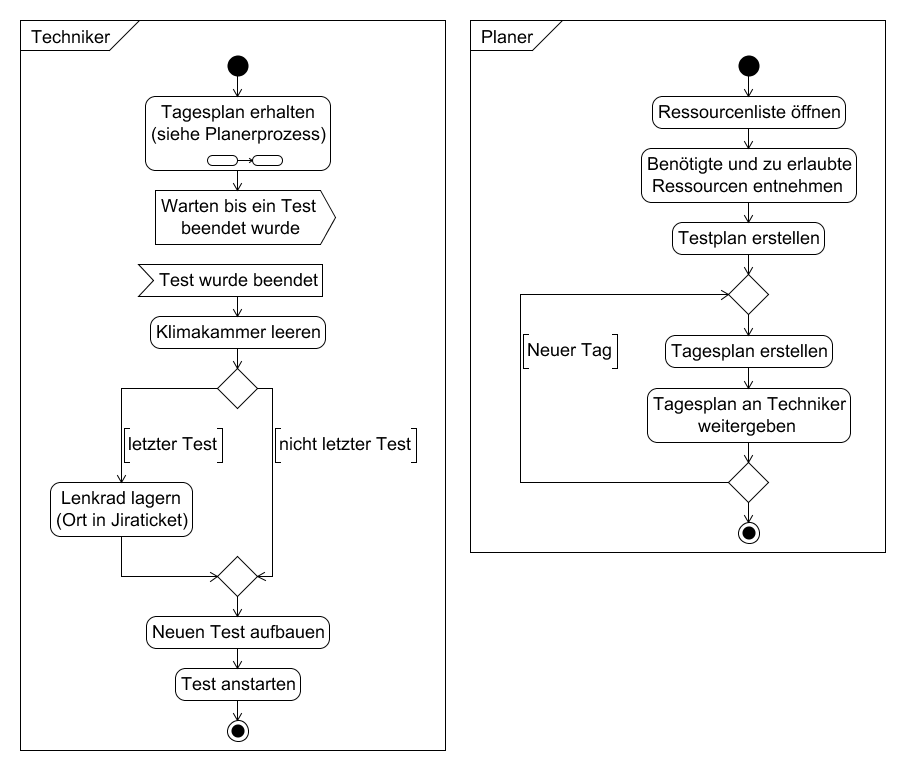
\includegraphics[width=\linewidth]{diagramme/TechnikerPlanerProzess.png}
    \caption{UML Aktivitätsdiagramm zum täglichen Testprozess}\label{fig:TechnikerPlanerProzess}
\end{figure}

Aus Abbildung~\ref{fig:TechnikerPlanerProzess} gehen zwei verschiedene Rollen hervor. Der
Planer (rechts) ist verantwortlich für das langfristige Planen von Tests. Dabei muss
dieser beachten, dass die Wartungstermine eingehalten werden, wenn
eine gewisse Ressource eingeplant wird. Welche Ressourcen überhaupt zur
Verfügung stehen und wann die Wartungstermine überhaupt sind, kann der Planer aus
der Ressourcenliste entnehmen. Zusätzlich erstellt der Planer auch den täglichen 
Tagesplan, welcher nur das Ergebnis eines \gls{JQL} Filters ist. 

Der Techniker (links) hingegen, ist für den Umbau und die tatsächliche Durchführung der 
Tests verantwortlich. Er benötigt den Tagesplan um zu wissen, welche Tests als 
nächstes durchgeführt werden. Da im Tagesplan allerdings nicht vermerkt ist, 
welcher Test nach eine spezifischen Test durchgeführt werden muss, muss er die 
Klimakammer so weit es nötig ist leeren, um anschließend den nächsten Test 
aufzubauen. Zusätzlich weiß er nicht, welcher Test der letzte einer Testgruppe ist.
Diese Information ist nötig, um die anschließende Lagerung des Lenkrads einzuleiten.
Um diese Information zu erhalten, muss er im jeweiligen Jira Ticket nachschauen. \\

\begin{figure}[H]
    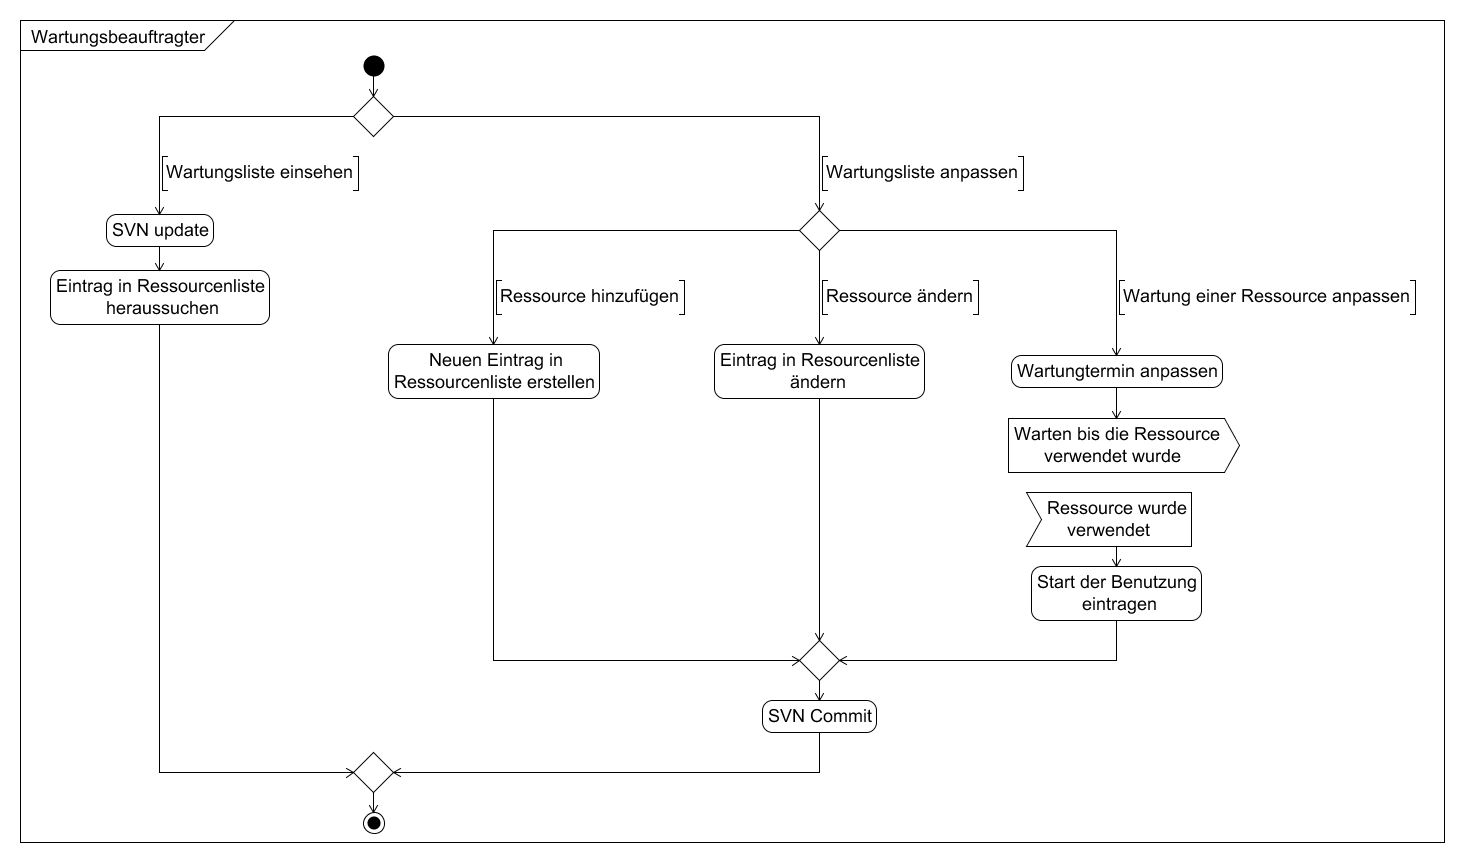
\includegraphics[width=\linewidth]{diagramme/WartungsbeauftragterProzess.png}
    \caption{UML Aktivitätsdiagramm zum Ressourcenmanagementprozess des Wartungsbeauftragten}\label{fig:WarterProzess}
\end{figure}

Der in Abbildung~\ref{fig:WarterProzess} beschriebene Prozess zeigt den Umgang mit der 
Ressourcenliste. Der Wartungsbeauftragte muss jedes mal, wenn er die Wartungsliste
einsehen will, vorher ein \gls{SVN} Update machen, um auch tatsächlich die aktuelle
Version der Liste zu erhalten. Wird dies nicht getan, kann es bei Änderungen 
zu \gls{SVN} Konflikten kommen oder die entnommenen Informationen sind veraltet.
Falls er irgendetwas an der Liste anpasst, muss diese anschließend wieder ins 
\gls{SVN} hochgeladen werden, um die Informationen mit allen anderen Mitarbeitern
zu synchronisieren. Zusätzlich muss zu jedem neuen Wartungstermin, das tatsächliche
Datum der ersten Benutzung seit der Wartung eingetragen werden.

Somit ergeben sich die folgenden Rollen:

\begin{description}
    \item[\textbf{Planer}] Die Rolle der Person, die Pläne für kurzfristige oder
    langfristige Tests erstellt.

    \item[\textbf{Wartungsbeauftragter}] Die Rolle der Person, die Wartungen 
    überwacht, plant und durchführt. 

    \item[\textbf{Techniker}] Die Rolle der Person, die Tests aufbaut, umbaut und
    durchführt
\end{description}

Auch wenn es sein kann, dass eine Person mehrere Rollen annimmt, ist es dennoch 
wichtig die Rollen voneinander zu unterscheiden um den Prozess nachvollziehbarer
und übersichtlicher zu gestalten.

\subsection{Einbindung in vorhandene Programme}
Da gerade die Wartungsinformationen auch in anderen Programmen benötigt werden, 
beispielsweise um Warnungen bei abgelaufener Wartungen bei der Testvorbereitung
anzeigen lassen zu können, ergibt sich eine weitere Rolle:

\begin{description}
    \item[\textbf{Entwickler}] Die Rolle der Person, die die Informationen der
    offenen Schnittstelle für eigene Programme verwendet
\end{description}

\subsection{Use Cases}\label{sec:usecases}
In Abbildung~\ref{fig:usecases} und Abbildung~\ref{fig:usecasesEntwickler} sind 
die bereits definierten Rollen als Akteure dargestellt.
Die Use Cases ergeben sich aus den Interviews.

\begin{figure}[H]
    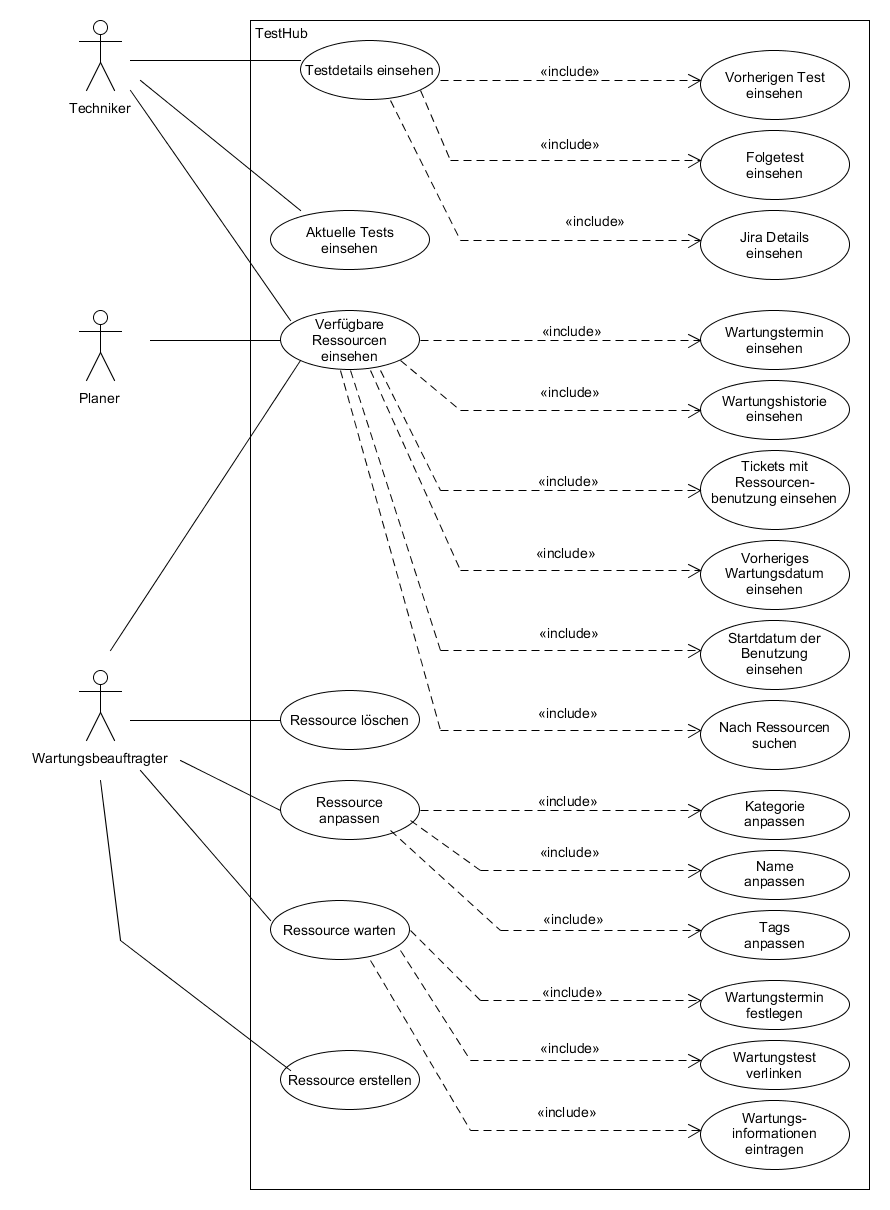
\includegraphics[width=\linewidth]{diagramme/Usecases.png}
    \caption{UML-Use-Case-Diagramm zu den Anwendungsfällen für die Planer-, Techniker- und Wartungsbeauftragten-Rolle}\label{fig:usecases}
\end{figure}

\begin{figure}[H]
    \includegraphics[width=\linewidth]{diagramme/UsecasesEntwickler.png}
    \caption{UML-Use-Case-Diagramm zu den Anwendungsfällen für die Entwickler-Rolle}\label{fig:usecasesEntwickler}
\end{figure}

\subsection{User Stories}\label{sec:userstories}
Die User Stories ergeben sich aus den Use Cases.

\begin{description}
    \descitem{US\#01}{itm:us01}
    \textit{Als Techniker möchte ich einen vorherigen Test einsehen}

    \descitem{US\#02}{itm:us02}
    \textit{Als Techniker möchte ich einen folgenden Test einsehen}

    \descitem{US\#03}{itm:us03}
    \textit{Als Techniker möchte ich die Details eines Jira-Tickets in 
    aufgeschlüsselter Form einsehen}

    \descitem{US\#04}{itm:us04}
    \textit{Als Techniker möchte ich alle aktiven Tests einsehen}

    \descitem{US\#05}{itm:us05}
    \textit{Als Techniker möchte ich eine schnelle Übersicht über die wichtigsten
    Ressourcen erhalten, um den Aufbau von Tests zu planen}

    \descitem{US\#10}{itm:us10}
    \textit{Als Planer möchte ich einen Wartungstermin einsehen, um zu erfahren
    ob ich diese Ressource einplanen kann}

    \descitem{US\#11}{itm:us11}
    \textit{Als Planer möchte ich eine Wartungshistorie einsehen, um eventuelle
    vergangene Probleme aufzudecken}

    \descitem{US\#12}{itm:us12}
    \textit{Als Planer möchte ich alle aktiven Tickets sehen, 
    welche eine spezifische Ressource verwenden}

    \descitem{US\#13}{itm:us13}
    \textit{Als Planer möchte ich das vorherige Wartungsdatum einsehen, 
    um zu wissen, ob das Startdatum der Benutzung hinter dem Wartungsdatum liegt
    und ich somit die Ressource verwenden kann}

    \descitem{US\#14}{itm:us14}
    \textit{Als Planer möchte ich das Startdatum der Benutzung einsehen,
    um zu wissen, ob das Startdatum der Benutzung hinter dem Wartungsdatum liegt
    und ich somit die Ressource verwenden kann }

    \descitem{US\#15}{itm:us15}
    \textit{Als Planer möchte ich nach Ressourcen suchen}

    \descitem{US\#20}{itm:us20}
    \textit{Als Wartungsbeauftragter möchte ich eine Ressource löschen}

    \descitem{US\#21}{itm:us21}
    \textit{Als Wartungsbeauftragter möchte ich die Kategorie einer Ressource anpassen}

    \descitem{US\#22}{itm:us22}
    \textit{Als Wartungsbeauftragter möchte ich den Namen einer Ressource anpassen}

    \descitem{US\#23}{itm:us23}
    \textit{Als Wartungsbeauftragter möchte ich die Tags einer Ressource anpassen}

    \descitem{US\#24}{itm:us24}
    \textit{Als Wartungsbeauftragter möchte ich einen neuen Wartungstermin festlegen}

    \descitem{US\#25}{itm:us25}
    \textit{Als Wartungsbeauftragter möchte ich das Ergebnis eines Wartungstest verlinken}

    \descitem{US\#26}{itm:us26}
    \textit{Als Wartungsbeauftragter möchte ich Informationen zu einer Wartung speichern}

    \descitem{US\#27}{itm:us27}
    \textit{Als Wartungsbeauftragter möchte ich eine Ressource erstellen}

    \descitem{US\#90}{itm:us90}
    \textit{Als Entwickler möchte ich die REST API verwenden, um die
    Informationen von ``TestHub'' in meine Programm einzubinden}

    \descitem{US\#91}{itm:us91}
    \textit{Als Entwickler möchte ich die Dokumentation
    der API ansehen, um zu verstehen wie ich die API benutzen kann}

\end{description}

\subsection{Funktionale Anforderungen}\label{sec:fas}
Um die Funktion der im Umfang dieser Arbeit entwickelten Software validieren zu
können, müssen Anforderungen definiert werden. Diese Funktionalen Anforderungen
werden in drei Kategorien eingeteilt:

\begin{description}
    \item[\textbf{Muss-Kriterien}]Die Kriterien die ``TestHub'' als \gls{MVP} zwingend erfüllen muss

    \item[\textbf{Soll-Kriterien}]Die Kriterien die für die Funktionalität von ``TestHub''
    nicht zwingend notwendig sind, aber dennoch implementiert werden sollten.

    \item[\textbf{Kann-Kriterien}]Die Kriterien, die rein optional sind. Da es sich
    bei ``TestHub'' um ein \gls{MVP} handelt, werden diese Kriterien nicht berücksichtigt.

\end{description}

Die folgenden Anforderungen ergeben sich aus den \nameref{sec:userstories} und den
in Abschnitt~\ref{sec:usecases} aufgezeigten Use Cases:

\begin{description}
    \descitem{FA\#01}{itm:fa01}
    \textit{TestHub muss den vorherigen und folgenden Test eines aktuell 
    ausgeführten Tests anzeigen können (\descref{US\#01}{itm:us01} \& \descref{US\#02}{itm:us02}).}\\
    Ein Test kann vorherige und folgende Tests haben, es gibt jedoch auch Tests,
    bei denen dies nicht der Fall ist.

    \descitem{FA\#02}{itm:fa02}
    \textit{TestHub muss die Informationen eines Jira-Tickets in übersichtlicher 
    Form anzeigen (\descref{US\#03}{itm:us03}).}

    \descitem{FA\#03}{itm:fa03}
    \textit{TestHub muss die Labels eines Jira-Tickets kategorisiert anzeigen (\descref{US\#03}{itm:us03}).}\\
    Die Labels eines Jira-Tickets liegen als simple Liste von Text vor. Dieser 
    Text soll analysiert und entsprechend kategorisiert werden, um eine genauere 
    Zuordnung zu ermöglichen.

    \descitem{FA\#04}{itm:fa04}
    \textit{TestHub muss alle aktiven Tests nach Klimakammer gruppiert anzeigen (\descref{US\#04}{itm:us04}).}\\
    Ein Test gilt als aktiv, wenn der Status seines Jira-Tickets ``Read for Test''
    oder ``In Execution'' ist.

    \descitem{FA\#05}{itm:fa05}
    \textit{TestHub muss eine schnelle Übersicht über die wichtigsten Ressourcen anzeigen (\descref{US\#05}{itm:us05}).}\\
    Die wichtigsten Ressourcen sind: aktive Tests, Ressourcen mit einem Wartungstermin
    in den nächsten 30 Tagen.

    \descitem{FA\#05}{itm:fa05}
    \textit{TestHub muss den nächsten Wartungstermin einer Ressource anzeigen (\descref{US\#10}{itm:us10}).}
    
    \descitem{FA\#06}{itm:fa06}
    \textit{TestHub muss die Wartungshistorie einer Ressource anzeigen (\descref{US\#11}{itm:us11}).}\\
    Die Wartungshistorie enthält alle Änderungen des Wartungstermins.

    \descitem{FA\#07}{itm:fa07}
    \textit{TestHub muss alle aktiven Tickets anzeigen, welche eine spezifische 
    Ressource verwenden (\descref{US\#12}{itm:us12}).}

    \descitem{FA\#08}{itm:fa08}
    \textit{TestHub muss das vorherige Wartungsdatum anzeigen (\descref{US\#13}{itm:us13} \& \descref{US\#11}{itm:us11}).}
    
    \descitem{FA\#09}{itm:fa09}
    \textit{TestHub muss das Startdatum der Verwendung einer Ressource anzeigen (\descref{US\#14}{itm:us14}).}\\
    Das Startdatum ist das Datum des Jira-Tickets welches nach dem Wartungstermin 
    der Ressource aktualisiert wurde und die Ressource verwendet.

    \descitem{FA\#10}{itm:fa10}
    \textit{TestHub muss die Suche nach Ressourcen unterstützen (\descref{US\#15}{itm:us15}).}
    
    \descitem{FA\#11}{itm:fa11}
    \textit{TestHub muss das löschen einer Ressource unterstützen (\descref{US\#20}{itm:us20}).}
       
    \descitem{FA\#12}{itm:fa12}
    \textit{TestHub muss das Anpassen der Kategorie einer Ressource unterstützen 
    (\descref{US\#21}{itm:us21}).}

    \descitem{FA\#13}{itm:fa13}
    \textit{TestHub muss das Anpassen des Namens einer Ressource unterstützen 
    (\descref{US\#22}{itm:us22}).}

    \descitem{FA\#14}{itm:fa14}
    \textit{TestHub muss das Anpassen der Tags einer Ressource unterstützen 
    (\descref{US\#23}{itm:us23}).}

    \descitem{FA\#15}{itm:fa15}
    \textit{TestHub muss Festlegen eines neuen Wartungstermins unterstützen 
    (\descref{US\#24}{itm:us24}).}

    \descitem{FA\#16}{itm:fa16}
    \textit{TestHub muss das Verlinken eines Wartungstests unterstützen 
    (\descref{US\#25}{itm:us25}).}

    \descitem{FA\#17}{itm:fa17}
    \textit{TestHub muss das Speichern weiterer wartungsspezifischer Informationen unterstützen 
    (\descref{US\#26}{itm:us26}).}

    \descitem{FA\#18}{itm:fa18}
    \textit{TestHub muss das Erstellen einer Ressource unterstützen 
    (\descref{US\#23}{itm:us23}).}\\
    Die Ressource benötigt mindestens einen Namen und sie muss nicht zwangsläufig 
    einen Wartungstermin haben.

\end{description}

\subsection{Nichtfunktionale Anforderungen}\label{sec:nfas}
Es ergeben sich folgende nichtfunktionale Anforderungen aus den Interviews und 
den User Stories:

\begin{description}
    \descitem{NFA\#01}{itm:nfa01}
    \textit{Die REST API von TestHub muss innerhalb der Firma verwendbar sein (\descref{US\#90}{itm:us90}).}

    \descitem{NFA\#02}{itm:nfa02}
    \textit{Die REST API von TestHub soll dokumentiert und erklärt werden (\descref{US\#91}{itm:us91}).}\\
    Es soll eine Website oder ein Dokument geben, in dem alle Endpunkte der REST API
    aufgelistet und erklärt sind. Des Weiteren soll es Beispiele zum 
    Verständnis geben.

    \descitem{NFA\#03}{itm:nfa03}
    \textit{TestHub soll die Verteilung der Jira-Tickets auf die einzelnen Projekte 
    aufzeigen (\descref{US\#05}{itm:us05}).}

    \descitem{NFA\#04}{itm:nfa04}
    \textit{Das \gls{UI} von TestHub soll ein einheitliches Design haben.}

    \descitem{NFA\#05}{itm:nfa05}
    \textit{TestHub muss in englischer Sprache verfügbar sein, da dies die 
    Firmensprache von JSS ist.}

    \descitem{NFA\#06}{itm:nfa06}
    \textit{TestHub muss unabhängig von den Jira Benutzerrechten für das HOD Projekt funktionieren}\\
    Da das System eine schnelle Übersicht schaffen soll und auch keine Möglichkeit
    bietet, Jira Daten anzupassen, soll das System die Jira Informationen unabhängig der Jira Rechte anzeigen.

    \descitem{NFA\#07}{itm:nfa07}
    \textit{TestHub muss mindestens auf den Webbrowsern ``Chrome'' und ``Edge'' funktionieren}\\
    Diese zwei Webbrowser werden innerhalb der Firma verwendet.

    
\end{description}

\section{Entwurf}\label{sec:entwurf}
Im folgenden Kapitel soll der Prozess der Gestaltung des \gls{UI}s erläutert 
werden. Des Weiteren wird die Architektur des \gls{Backend}s und einiger Komponenten
genauer beschrieben.

\subsection{Entwurf des GUI}
Im folgenden Abschnitt wird das Grundlegende Design kurz erläutert. AnschließenD
wird auf den Aufbau und Entwurf der zwei Haupt-Webseiten von ``TestHub'' eingegangen. 

Da ``TestHub'' im Browser auf verschiedenen Bildschirmen laufen wird, muss das 
Design auch eine gewisse ``Responsiveness'' haben, was bedeutet, dass sich die 
GUI dem Viewport anpasst.

\subsubsection{Grunddesign}\label{sec:grunddesign}
Um das in \descref{NFA\#21}{itm:nfa21} angesprochene einheitliche Design umzusetzen, 
wurde ein simples Design erstellt, welches sich im gesamten Projekt wiederfinden
lässt. Das Design basiert auf ``Karten'' welche sich leicht entwerfen lassen und
zudem übersichtlich und skalierbar sind.

\begin{figure}[H]
    \includegraphics[width=\linewidth]{img/KartenDesign.png}
    \caption{Finales Kartendesign}\label{fig:card}
\end{figure}

Das Kartendesign wurde mit dem Designtool Figma\footurl{https://www.figma.com} erstellt. Jede Karte besitzt 
einen Header welcher die Hintergrundfarbe \textit{\#1f2937} besitzt. In diesem
Header lassen sich der Karten Titel und ein Button wiederfinden.
Der Titel der Karte sollte dabei immer eine kurze Beschreibung des Inhalts sein.
Der Button in der rechten Ecke des Headers its optional und kann beliebig 
angepasst werden. Der Body der Karte lässt platz für alle beliebigen Elemente.
Durch das simple Design sind die Höhe und Breite der Karte variabel, wodurch 
jedes beliebige Element im Body platz findet. Um die Benutzererfahrung zu verbessern,
wird beim Hovern über der Karte, diese in einer Animation etwas nach oben verschoben. 
Zusätzlich wird der Schatten der Karte vergrößert, sodass sie einen Anhebe-Effekt
erhält, welcher jedoch nicht zu ablenkend ist.

\subsubsection{Entwurf einer kompakten Jira-Ticket Komponente}\label{sec:jirakompakt}
Da es Sinn macht, vorherige und folgende Tests zusammen mit dem aktiven Test 
anzuzeigen, wurde ein Element entworfen, welches die wichtigsten Informationen 
des Tickets in kompakter Weise anzeigt und trotzdem die Möglichkeit bietet, den 
vorherigen und folgenden Test einzusehen.
Durch die Verwendung von TailwindCSS konnte die Komponente schnell und einfach 
direkt in \gls{HTML} entworfen werden. Dadurch lässt sie sich auch leichter in
das fertige Projekt einbauen.

\begin{figure}[H]
    \includegraphics[width=\linewidth]{img/TicketKompakt.png}
    \caption{Kompakte Jira-Ticket Komponente}\label{fig:ticketcompact}
\end{figure}

In dem Design dieser Komponente lassen sich die wichtigsten Ticket Informationen
auf einen Blick erkennen, wie in~\descref{FA\#02}{itm:fa02} gefordert. 
Falls man dennoch das ganze Jira-Ticket ansehen möchte,
kann dies über die Verlinkung der Ticket-ID (Abb.~\ref{fig:ticketcompact}, Nr. 1) geschehen. Des Weiteren sieht man in 
dieser Komponente auch schnell, falls ein Test der letzte Test ist (Abbildung
~\ref{fig:ticketcompact} Nr. 3). Klickt man auf eine freie Stelle innerhalb
der Komponente, soll sich die Detailansicht des Tickets öffnen, klickt man auf 
den Knopf des vorherigen oder folgenden Tests, soll sich die Detailansicht des 
entsprechenden Tickets öffnen. Weiterhin lässt sich durch die geringe Höhe der 
Komponente eine kompakte Auflistung mehrerer Tickets ermöglichen.

\subsubsection{Dasboard}
Um die in \descref{FA\#05}{itm:fa05} geforderte schnelle Übersicht zu entwerfen, 
wurde zuerst analysiert, welche Daten angezeigt werden müssen. Wie in der 
Anforderung \descref{FA\#05}{itm:fa05} beschrieben müssen sowohl die aktiven Jira-Tickets als auch 
aufkommende Wartungen angezeigt werden. All diese Informationen sollen auf dem 
``Dashboard'' übersichtlich dargestellt werden. Das Dashboard soll gleichzeitig
die Hauptseite des Projekts sein.

\begin{figure}[H]
    \includegraphics[width=\linewidth]{img/DashboardMockUp.png}
    \caption{MockUp des Dashboards}\label{fig:dashboard}
\end{figure}

In Abbildung~\ref{fig:dashboard} ist ein Mockup des Dashboards zu sehen. 
Die Entwicklung des Dashboards folgte einem iterativen Prozess. Das Mockup wurde
den betroffenen Personen vorgestellt und in mehreren Schritten verfeinert, indem die 
Rückmeldungen der Befragten implementiert wurden.\\

Das Dashboard benutzt das in Abschnitt~\ref{sec:grunddesign} gezeigte Kartendesign.
Dabei wird das Dashboard in drei Spalten aufgeteilt, welche die aktiven Tests nach
Klimakammer gruppiert (Abb.~\ref{fig:dashboard}, Nummer 1), 
die aufkommenden Wartungen (Abb.~\ref{fig:dashboard}, Nummer 2) und eine 
Projektübersicht (Abb.~\ref{fig:dashboard}, Nummer 3) bietet. In den Klimakammerkarten
lässt sich auch die in Abschnitt~\ref{sec:jirakompakt} gezeigte kompakte Jira-Ticket 
Komponente wiederfinden. \\

Da es für die Jira-Tickets viele weitere interessante Informationen gibt, welche
jedoch sich nicht in einer kompakten Ansicht anzeigen lassen, gibt es für jedes
aktive, vorherige und folgende Ticket eine Detailansicht. Damit wird sowohl die
funktionale Anforderung \descref{FA\#02}{itm:fa02} als auch \descref{FA\#03}{itm:fa03} erfüllt.
Die Detailansicht wird durch ein Modal umgesetzt. Ein Modal ist ein Dialog, welcher den Rest der Anwendung sperrt,
bis das Modal wieder geschlossen wird.

\begin{figure}[H]
    \includegraphics[width=\linewidth]{img/TicketModal.png}
    \caption{MockUp des Modals zur anzeige von Jira-Ticket Details}\label{fig:modal}
\end{figure}

In Abbildung~\ref{fig:modal} werden nur einige der Labelkategorien angezeigt.
Falls es nicht möglich ist, ein Label zu kategorisieren, wird dieses ganz unten 
unter ``Unknown Labels'' angezeigt. 

\subsubsection{Ressourcendetailansicht}
Um die Details einer Ressource einzusehen und diese zu bearbeiten muss es eine 
extra dafür angefertigte Seite geben. 

\begin{figure}[H]
    \includegraphics[width=\linewidth]{img/RessourceMockUp.png}
    \caption{MockUp der Ansicht einer spezifischen Ressource}\label{fig:ressource}
\end{figure}

Auch in dieser Ansicht lässt sich das Design aus Abschnitt~\ref{sec:grunddesign}
wiederfinden. Das~\nameref{fig:ressource} liefert alle wichtigen Informationen
auf einen Blick. Viele dieser Informationen lassen sich auch interaktiv anpassen
und mit dem ``Save'' Button übernehmen. Die Kategorien und Tags zeigen bei Benutzung
des jeweiligen Eingabefeldes, die schon vorhandenen Kategorien oder Tags des Servers
an, um die Eingabe so bequem wie möglich zu machen. \\

Unter der Equipment Karte, befinden sich noch zwei weitere Karten. Die linke Karte
zeigt dabei die in \descref{FA\#22}{itm:fa22} geforderten Tickets, welche die 
entsprechende Ressource verwenden. In Abbildung~\ref{fig:ressource} unter Nr. 7 sieht man die Ansicht,
wie sie aussieht, wenn es keine solcher Tickets gibt. Falls es diese doch Tickets gibt, 
wird die Klimakammeransicht aus Abbildung~\ref{fig:dashboard} Nr. 1 erneut verwendet,
um die Tickets anzuzeigen.

Mit dem ``Update'' Button kann ein neuer Wartungstermin erstellt werden.
Es öffnet sich erneut ein Modal wo die in \descref{FA\#11}{itm:fa11}, 
\descref{FA\#30}{itm:fa30} und \descref{FA\#31}{itm:fa31} geforderten wartungsspezifischen
Informationen eingetragen und abgespeichert werden können. Dadurch wird ein neuer
Wartungstermin festgelegt und ein Wartungsverlaufeintrag erstellt.


\subsection{Entwurf der Softwarearchitektur}\label{sec:swArchitectur}
Im Kapitel~\ref{sec:swArchitectur} wird die Architektur der Software detailliert 
erläutert. Zusätzlich werden alle Systemkomponenten erklärt und auf die 
Datenmodellierung eines Jira-Tickets erläutert. Zum Schluss wird auf die Struktur
der \gls{UI}-Komponenten eingegangen.

\subsubsection{Systemarchitektur}
Das System ist in dem klassischen Server-Client-Prinzip aufgebaut, in dem der Server, 
als \gls{Backend}, die nötigen Daten zur Verfügung stellt und der Client diese 
abfragen kann um seine spezifischen Aufgaben zu lösen~\cite{Nie13}.
In diesem Fall ist der Client der Webbrowser mit dem der Benutzer interagiert. 
Die Server-Komponente, stellt die Daten aus der Datenbank oder dem \gls{Jira} Server
zur Verfügung. Der Server dient auch als Webserver, indem er ebenfalls die
\gls{HTML}, \gls{CSS} und Javascript Dokumente zur Verfügung stellt.\\

\begin{figure}[H]
    \includegraphics[width=\linewidth]{diagramme/KomponentenDiagramm.png}
    \caption{UML-Komponentendiagramm zur Systemarchitektur}\label{fig:components}
\end{figure}

In Abbildung~\ref{fig:components} sind die genannten Komponenten visuell dargestellt.
Die dick geschriebenen Komponenten sind in dieser Arbeit entwickelt worden, alle
anderen werden nur als Quellen genutzt, um Daten zu erhalten oder Interaktionen zu 
ermöglichen. Dadurch ergeben sich 3 Hauptkomponenten:

\begin{description}
    \descitem{GUI}{itm:GUI}\hfill\\
    Die Grafische Benutzeroberfläche mit der der Benutzer interagieren kann.
    Die \gls{GUI} wird durch strukturell durch \gls{HTML} Dokumente ermöglicht. 
    Das Design wird dabei durch TailwindCSS\footurl{https://tailwindcss.com} umgesetzt.

    \descitem{Server}{itm:server}\hfill\\
    Der Server bietet über eine \gls{REST} \gls{API} (siehe Abs.~\ref{sec:restapi})
    die vom Client benötigten Daten an. Der Server kann dabei eine Vielzahl an Clients
    gleichzeitig bearbeiten.

    \descitem{Controller}{itm:controller}\hfill\\
    Der Controller verarbeitet die Daten des Servers, sodass sie in der GUI
    dargestellt werden können. Er ist ein eigenes JavaScript Programm,
    welches vom Browser ausgeführt wird.\\
\end{description}

Zusätzlich gibt es zwei weitere Komponenten mit denen der Server interagiert:

\begin{description}
    \descitem{Jira Server}{itm:jiraserver}\hfill\\
    Der \gls{Jira} Server ist der Server auf dem das Programm \gls{Jira} ausgeführt wird, 
    welches die Informationen zu allen Tests beinhaltet.

    \descitem{Datenbank}{itm:datenbank}\hfill\\
    Die Datenbank dient als zweite Informationsquelle. In ihr speichert der Server
    die Daten der Ressourcen, welche üblicher Weise nicht durch \gls{Jira} verwaltet
    werden.
\end{description}

Die Kommunikation der Komponenten erfolgt auf unterschiedliche Weisen. Während 
der Controller mit der GUI über das vom Browser zur Verfügung gestellte \gls{DOM}
Interface interagiert, kommuniziert er mit dem Server via \gls{HTTP} (siehe \nameref{sec:HTTP}).
Der Server fragt seine Daten ebenfalls über HTTP vom \gls{Jira} Server an. Um Einträge
in der Datenbank zu speichern, anzupassen oder abzufragen wird die Query-Sprache
der Datenbank verwendet.

\begin{figure}[H]
    \includegraphics[width=\linewidth]{diagramme/SequenzDiagramm.png}
    \caption{UML-Sequenzdiagramm zur Anfrage der aktiven Tickets bei Initialisierung}\label{fig:sequenz}
\end{figure}

In Abbildung~\ref{fig:sequenz} ist die Kommunikation beim Laden der aktiven Tickets des Dashboards 
dargestellt. Da sich der Ablauf immer ähnelt, nur der rechte Teilnehmer, je nach 
Anfrage die Datenbank ist, kann man dieses Prinzip auf die Kommunikation des gesamten
Systems beziehen. Der Server ist demnach nur eine Zwischenkomponente, welche die
Daten einheitlich, gesammelt und aufbereitet wiedergibt.

Aus Übersichtlichkeitsgründen wurde die \descrefnobold{GUI}{itm:GUI}
und der \descrefnobold{Controller}{itm:controller} als Client zusammengefasst.\\

\subsubsection{\gls{Jira} Ticket Modellierung}
Ein JiraTicket ist im Backend wie in Abbildung~\ref{fig:classes} strukturiert. Die Struktur ist abgeleitet 
von dem \gls{JSON}-Dokument, welches der \gls{Jira} Server versendet. Der \gls{Jira} Server
sendet noch viele weitere Informationen zu einem Ticket, welche aufgrund der Relevanz
nicht beachtet werden.

\begin{figure}[H]
    \includegraphics[width=\linewidth]{diagramme/KlassenDiagramm.png}
    \caption{UML-Klassendiagramm zur Jira-Ticket Struktur}\label{fig:classes}
\end{figure}

In Abbildung~\ref{fig:classes} ist zu sehen, dass ein JiraIssue hauptsächlich aus 
seinen ``Field''-Attributen besteht. Diese decken sich größtenteils mit der 
\gls{JSON} Repräsentation des \gls{Jira} Tickets. Sie wurde lediglich um die ParsedLabels Struktur 
erweitert, um die Labels in aufgeschlüsselter Form anzuzeigen (siehe \descref{FA\#03}{itm:fa03}). Dafür wird auch die
öffentliche Methode \textit{ParseLabels} eingeführt, welche das Parsen, also das
Analysieren und Kategorisieren durchführt. 

In den ``Field''-Attributen lassen sich auch die Verlinkungen wiederfinden, falls 
es welche gibt. Diese Verlinkungen werden durch eine eigene Struktur realisiert.
Dabei erhält jeder Link eine ID, die Art der Verlinkung und einen Inward- \textit{oder}
einen Outward-Issue. ``Inward'' bedeutet in diesem Fall, dass ein anderes Ticket auf dieses
Ticket verlinkt, ``Outward'' beschreibt hingegen die ausgehende Verlinkung vom Ticket aus. 
Um riesige Baumstrukturen durch die Verlinkungen zu vermeiden, 
ist zwar der Inward- bzw. Outward-Issue ein Objekt der JiraIssue Klasse, jedoch 
werden in dem verlinken Ticket nur eine geringe Anzahl der Felder mit Werten befüllt.
Des Weiteren hat das verlinkte Ticket nie weitere Verlinkungen.

Die jeweilige Art der Verlinkung wird in der separaten 
``JiraIssueLinkType'' Struktur festgehalten. Dort findet man auch die Beschreibung
der Beziehung zwischen den Tickets in Worten. Durch diese Verlinkungsstruktur
lassen sich die vorherigen und folgenden Tests, wie in \descref{FA\#04}{itm:fa04}
gefordert, ermitteln.

Nicht nur für die Verlinkung gibt es extra Strukturen, auch der Status, das Projekt, 
die Testklasse und Accounts werden in eigenen Strukturen betrachtet, um weitere
Informationen zu dem jeweiligen Feld zu liefern.

Das Parsen zu oder von der \gls{JSON} Repräsentation kann in GO sehr leicht über
sogenannte ``Tags'' realisiert werden. Somit kann bei der Deklaration der Struktur
direkt der \gls{JSON}-Key mit angeben werden, welcher zur (De)Serialisierung verwendet wird.

\begin{lstlisting}[caption=Go Strukturdefinition mit JSON Tags,language=Go]
type JiraIssue struct {
    ID     string     `json:"id"`
    Key    string     `json:"key"`
    Fields JiraFields `json:"fields"`
}
\end{lstlisting}

Ein in \gls{JSON} serialisiertes Jira-Ticket, beispielsweise im Body einer Antwort
des Servers, sieht wie folgt aus:

\begin{lstlisting}[caption=gekürzte beispielhafte JSON Repräsentation eines Jira-Tickets,language=json,label={lst:jirajson}]
{
    "id": "12345",
    "key": "C3000000-1234",
    "fields": {
        "labels": [
            "Au123",
            "HW:123",
            "RBS:1.2.3",
            "SW:321",
            "heated"
        ],
        "parsed_labels": {
            "arduino_sw": "Au123",
            "ecu_hw": "HW:123",
            "ecu_sw": "SW:321",
            "heated": true,
            "restbus_sim": "RBS:1.2.3",
            "last_test": false,
            "unknown_labels": null,
            // ...
        },
        "description": "Please perform TCSY000",
        "created": "2022-03-09T08:27:41.000+0100",
        "updated": "2022-03-23T13:34:59.000+0100",
        "assignee": {
            "name": "paellern",
            "key": "paellern",
            "displayName": "Nico Paeller",
            "emailAddress": "nico.paeller@joysonsafety.com",
            "avatarUrls": {
                // ...
            }
        },
        "status": {
            "id": "10900",
            "name": "Ready for Test",
        },
    }
}
\end{lstlisting}

Diese \gls{JSON}-Repräsentation eines Jira-Tickets wurde gekürzt, um die Übersichtlichkeit
dieses Dokuments zu erhalten. \\

In Codebeispiel~\ref{lst:jirajson} können auch die Labels im Vergleich zu den
``ParsedLabels'' gesehen werden.

\subsubsection{Komponentenarchitektur}
Die einzelnen Komponenten wurden nach der \gls{MVC}-Architektur entworfen. Unter
Komponenten sind hier die Views, also die einzelnen Webseiten (Dashboard, etc.) 
von TestHub gemeint.

\begin{figure}[H]
    \includegraphics[width=\linewidth]{diagramme/MVC.png}
    \caption{UML-Klassendiagramm zur Jira-Ticket Struktur}\label{fig:classes}
\end{figure}

Das Projekt ist also in drei Teile unterteilt:
\begin{description}
    \descitem{Model}{itm:model}\hfill\\
    Das Model beinhaltet die Informationen, welche dargestellt werden sollen. Das
    Model ist im Fall von ``TestHub'' der Server, welcher die Daten zur Verfügung stellt.

    \descitem{View}{itm:view}\hfill\\
    Das View übernimmt die Anzeige der Daten an den Benutzer. Es kann zusätzlich
    verschiedene Methoden zur Verfügung stellen, um Benutzereingaben an den Controller
    weiter zu geben. Bei TestHub ist das View das Zusammenspiel aus \gls{HTML} und \gls{CSS}.

    \descitem{Controller}{itm:mvcController}\hfill\\
    Der Controller stellt die Schnittstelle zwischen View und Model her. Er kann 
    auf Eingaben vom View reagieren und entsprechende Models laden und anzeigen lassen.
    Der Controller wird durch die JavaScript/TypeScript Programme umgesetzt.
\end{description}

Durch diese Architektur bleibt das Projekt übersichtlich gegliedert und erweiterbar, 
da einzelne Views, Controller oder Models ausgetauscht werden und somit eine andere 
Darstellung oder Funktionalität bieten können~\cite{Aug20}. Des Weiteren ist das Projekt so 
aufgebaut, dass der einzige Punkt, wo View und Controller zusammengeführt werden,
das Laden des jeweiligen Skripts im \gls{HTML} Head ist. Da es keine weiteren 
Funktionsaufrufe oder Ähnliches im \gls{HTML} Dokument gibt, kann der Controller
aufgebaut und Design werden, wie es nötig ist. \\

Die schemenhafte Umsetzung dieser Architektur lässt sich in Abbildung~\ref{fig:components}
wiederfinden.

\newpage

\section{Entwicklung}
In diesem Kapitel wird die Umsetzung des in Kapitel~\ref{sec:entwurf} besprochenen
Entwurfs erläutert. Es wird nicht nur auf den Projektaufbau und die Implementierung 
von \gls{Frontend} und \gls{Backend} eingegangen, sondern auch auf den 
Softwarelebenszyklus des Projekts und die Dokumentation der \gls{REST} \gls{API}.

\subsection{Projektaufbau}
Das Projekt wurde als ``Monorepo'', also als allumfassendes Repository, entwickelt.
Dadurch sind alle für TestHub benötigten Dateien am gleichen Ort. Weiterhin muss 
keine Synchronisation der Frontend und Backend Versionen stattfinden, was den
Entwicklungs- und Update-Prozess erleichtert~\cite{PL16}.

Dennoch kann das Projekt in zwei interne Teile aufgeteilt werden:

\begin{description}
    \descitem{Frontend}{itm:frontend}\hfill\\
    Unter das Frontend fallen alle vom Client ausgeführten Dateien. Unter das Frontend
    fallen nicht nur die Dateien im \textit{frontend/src} Ordner, wo sich die 
    Controller Dateien befinden, sondern auch alle Dateien in \textit{static/} (kompiliertes JavaScript/CSS) 
    und \textit{templates/} (HTML Dateien).

    \descitem{Backend}{itm:backend}\hfill\\
    Das Backend beschreibt das serverseitige Program, welches auch die \gls{REST} \gls{API}
    implementiert. Der Quellcode dazu liegt im \textit{backend/} Ordner.
\end{description}

Im \textit{frontend/src/} Ordner lassen sich Quellcode für den Style Sheet und 
die Controller finden. Der finale Style Sheet wird mittels TailwindCSS\footurl{https://tailwindcss.com}
kompiliert, welches den Quellcode der HTML und TypeScript Dateien analysiert und
die darin verwendeten \gls{CSS} Klassen generiert. Die Controller hingegen, wurden alle mit 
TypeScript\footurl{https://www.typescriptlang.org} erstellt, welches, im Gegensatz zu 
JavaScript, Typisierung, Interfaces und vieles mehr ermöglicht. Die TypeScript Dateien 
werden in einen einstellbaren JavaScript Standard, wie zum Beispiel ``es2016''
kompiliert. Alle Kompilate werden im \textit{static/} Ordner unter der gleichen 
Struktur gespeichert.

Das Projekt wurde gänzlich im Dateieditor Visual Studio Code\footurl{https://code.visualstudio.com}
unter Verwendung der Go und der JavaScript und TypeScript Extension entwickelt.

\subsection{Implementierung des Frontends}
In diesem Abschnitt wird anhand eines Beispiels aus dem Projekt, die Umsetzung
asynchroner Anfragen erläutert.

\subsubsection{Asynchrones Laden aktiver Jira-Tickets}
Um das Laden der aktiven Tickets so schnell wie möglich zu gestalten, werden die
Tickets asynchron, also pseudo-parallel geladen. Dies wird zum einen möglich, durch
die intuitiv benutzbare Fetch API\footurl{https://developer.mozilla.org/en-US/docs/Web/API/Fetch\_API/Using\_Fetch}
von JavaScript, welche eine einfache asynchrone Umsetzung von Anfragen ermöglicht.
Zum Anderen, kann die Anzahl der angeforderten Tickets durch sogenannte Pagination
limitiert und eingestellt werden. Pagination ist die Möglichkeit, den Umfang 
der angefragten Ressourcen zu limitieren.

\begin{lstlisting}[caption=TypeScript Funktion zum asynchronen Laden aktiver Tickets (\textit{frontend/src/ts/dashboard.ts}),language=TypeScript]
const issueAmount = 20

function loadClimateChamberWidget(){
    var total = 0
    var request_amount = 0

    api<JiraGroupedCCQueryResult>(
        `/jira/active?grouped=true&startAt=0&maxResults=${issueAmount}`
    ).then(res => {
        // first api request to also get the total amount of issues
        total = res.totalResults
        request_amount = res.startAt + res.maxResults
        storeClimateChamber(res.data)
        
        // multiple async requests to load the data faster
        for (
            let i = issueAmount*2;
            i < res.totalResults;
            i+=issueAmount
        ) {
            api<JiraGroupedCCQueryResult>(
                `/jira/active?grouped=true&startAt=${i}&maxResults=${issueAmount}`
            ).then(res => {
                storeClimateChamber(res.data)
            })
        }
    })  
}
\end{lstlisting}

In der Funktion \textit{loadClimateChamberWidget} wird zuerst eine GET Anfrage an die \gls{API} gesendet.
Das Ergebnis ist ein Objekt, welches dem Interface \textit{JiraGroupedCCQueryResult} entspricht.
Die Anfrage wird an die \gls{URI} \textit{/jira/active} gesendet, wobei noch einige optionale 
Formwerte angegeben werden:

\begin{description}
    \item[grouped]
    Angabe, ob die aktiven Tickets vom Server, so wie in \descref{FA\#01}{itm:fa01}
    gefordert, nach Klimakammer sortiert werden sollen.

    \item[startAt]
    Der Startindex, ab welchem die Tickets in der Antwort enthalten werden sollen. In der ersten 
    Anfrage an den Server (Zeile 8) sollen alle Tickets ab dem ersten empfangen werden.

    \item[maxResults]
    Die Anzahl der Tickets, die maximal empfangen werden soll. In der ersten 
    Anfrage an den Server (Zeile 8) sollen maximal 20 Tickets empfangen werden.
\end{description}

Die Antwort des Servers enthält demnach nicht nur die Tickets, sondern auch Informationen
zum Requests, wie die eben genannten \textit{startAt} und \textit{maxResult} Werte
aber auch die Anzahl der gesamten verfügbaren Tickets.

Wenn eine Antwort empfangen wurde, werden weitere Anfragen dieser Art verschickt, mit inkrementiertem \textit{startAt} Wert.
Durch die asynchrone Eigenschaft der \textit{fetch} Funktion (innerhalb der \textit{api} Funktion),
wird nicht auf die Antwort einer Anfrage gewartet bis man die Nächste startet.
Stattdessen können weitere Anfragen gestartet werden, während auf andere Antworten gewartet wird.
Durch diese Umsetzung lässt sich ein wesentlich schnelleres Laden der Jira-Tickets ermöglichen .

\subsection{Implementierung des Backends}
In diesem Abschnitt werden ausgewählte Teile des Backendquellcodes vorgestellt.
Dabei wird nicht nur auf die Umsetzung der Kategorisierung anhand eines Beispiels eingegangen,
sondern auch auf die Kommunikation mit dem \gls{Jira} Server.

\subsubsection{Kategorisieren der Jira Labels}
Das Kategorisieren der Labels wird durch reguläre Ausdrücke (englisch: Regular 
Expressions; kurz: RegEx) umgesetzt. Mit diesen kann der strukturelle Aufbau 
von Text schnell analysiert werden~\cite{fitzgerald2012einstieg}. Da reguläre
Ausdrücke sehr schnell sehr unübersichtlich werden können, wurde zu jedem 
RegEx String ein entsprechender Link zu Regex101.com erstellt, in welchem der String
analysiert, erklärt und getestet werden kann.\\

Im Folgenden wird beispielhaft ein RegEx String für ein Erdungskabel kurz gezeigt 
und aufgeschlüsselt erklärt:

\begin{center}
    \verb@(?i)^gc(_|-)?\d+$@
\end{center}

Die ID eines Erdungskabel hat das Format: GC\_100. Jedoch gibt es, durch das manuelle
Eintragen der ID, häufig andere Variationen dieser ID, welche vom Programm 
dennoch als Erdungskabel kategorisiert werden sollen. Beispiele dieser Variation wären: GC100, gc\_100, GC-100, GC\_0100.
Durch den RegEx String können all diese Formate schnell und ohne viel Quellcode 
erkannt werden. Obwohl der String anfangs recht kompliziert aussieht, lässt er 
sich sehr leicht erklären\footurl{https://pkg.go.de/regexp/syntax}:

\begin{table}[H]
    \centering
    \begin{tabular}{| P{0.2\linewidth} | P{0.5\linewidth} | P{0.2\linewidth} |} 
        \hline
        \textbf{Substring} & \textbf{Erklärung} & \textbf{Beispiel}\\ [0.5ex] 
        \hline
        \verb@(?i)@ & Case-insensitive flag; ignoriert Groß- und Kleinschreibung & - \\ [0.5ex]
        \hline
        \verb@^@ & String muss mit folgendem Zeichensatz beginnen & - \\ [0.5ex] 
        \hline
        \verb@gc@ & akzeptiert nur die Buchstaben ``g'' und ``c'' in dieser Reihenfolge & \textbf{\textcolor{blue}{GC}}\_100 \\ [0.5ex] 
        \hline
        \verb@(_|-)@ & akzeptiert entweder ``\_'' oder ``-'' & GC\textbf{\textcolor{blue}{\_}}100 \\ [0.5ex] 
        \hline
        \verb@?@ & das vorherige Zeichen oder Gruppe darf maximal 1 mal vorkommen & - \\ [0.5ex] 
        \hline
        \verb@\d+@ & akzeptiert nur Zahlen (mindestens eine durch \textbf{+}) & GC\_\textbf{\textcolor{blue}{100}}\\ [0.5ex] 
        \hline
        \verb@$@ & String muss mit vorherigem Zeichensatz enden & - \\ [0.5ex] 
        \hline
    \end{tabular}
    \caption{Aufschlüsselung des regulären Ausdrucks zum Identifizieren einer Erdungskabelstruktur in einem String}
\end{table}

Wenn also die \textit{ParseLabels} Methode eines Jira-Tickets aufgerufen wird, werden
alle Labels nacheinander auf das Passen der Struktur mit einem der definierten ReGex Strings geprüft.
Falls ein Label zu einer gewissen Struktur passt, wird es in das entsprechende \textit{ParsedLabel}
geschrieben. Durch das Kompilieren der ReGex Strings beim Start des Servers, können 
diese so schnell wie möglich die Labels kategorisieren.

\subsubsection{\gls{Jira} Kommunikation}
Das TestHub Backend kommuniziert mit dem \gls{Jira} Server via \gls{HTTP}. Dabei muss 
jede Anfrage eine Authentifizierung im Header mitschicken. Diese Authentifizierung
wird durch den Benutzernamen und das Passwort als Base64 kodierter String ermöglicht.
Diese Methode ist zwar nicht sehr sicher, gerade über eine unverschlüsselte
Verbindung wie \gls{HTTP}, allerdings gibt es, da es keine OAuth Authentifizierung auf
dem \gls{Jira} Server von \gls{JSS} bereitgestellt wird, keine andere Möglichkeit.
Allerdings ist der \gls{Jira} Server nur im Firmennetzwerk erreichbar, was das Sicherheitsrisiko
durch Dritte, die eventuell sensible Daten, wie das Passwort, mitlesen, verringert.

Um die in \descref{NA\#13}{itm:fa13} geforderte Funktionalität umzusetzen, 
wird ein standard Jira-Account verwendet, der die Rechte zu den benötigten Projekten besitzt.
Die Zugangsdaten werden aus Sicherheitsgründen nicht direkt in den Quellcode geschrieben, 
sondern über Umgebungsvariablen gelöst. Solch eine Umgebungsvariable ist eine Variable, 
welche Werte zur Laufzeit eines Programms bereitstellen kann. Sie wird meistens vom Betriebssystem verwaltet.
Durch diese Lösung, existieren die Accountdaten nur auf dem Rechner, wo sie auch
angelegt wurden und können nicht einfach so und geteilt oder von Außen eingesehen werden.
Da es jedoch, je nach Betriebssystem, etwas mühselig ist, Umgebungsvariablen zu
verwalten, verwendet TestHub eine \textit{.env} Datei, welche zur Laufzeit eingelesen
wird und die darin enthaltenen Variablen als Umgebungsvariablen setzt. Diese Datei
wird demnach auch nie in das Versionskontrollsystem aufgenommen und kann trotzdem
leicht unter Entwicklern geteilt werden.

\paragraph{Asynchrone Kommunikation}\hfill\\
Das Kreieren einer asynchronen Funktion in Go ist prinzipiell sehr leicht umsetzbar.
Dazu muss lediglich das \textit{go} Keyword vor eine Funktion geschrieben werden.
Dadurch wird die Funktion in einer Go Routine ausgeführt, welche mit einem Thread 
des Betriebssystems vergleichbar ist. 
Jedoch ist das Problem bei der Entwicklung, dass der Server, wie in Abbildung~\ref{fig:components}
dargestellt, zwischen Client und Server liegt. Daher muss, nachdem der Client 
eine entsprechende Anfrage geschickt hat, der TestHub Server die Daten vom \gls{Jira} 
Server so schnell wie möglich lesen und in der gewünschten Form an den Client zurücksenden.
Werden die Anfragen von TestHub an \gls{Jira} jedoch in einer Go Routine ausgeführt, wird logischer Weise nicht
auf die Antwort des \gls{Jira} Servers gewartet, bis die nächste Zeile Code ausgeführt wird.
Dadurch würde TestHub dem Client mit einem leeren Datensatz antworten.

Aus diesem Grund müssen diese Anfragen weiterhin asynchron verschickt werden, um den Geschwindigkeitsbonus
beizubehalten, jedoch muss auf jede Jira-Antwort gewartet werden, bis TestHub an
den Client eine Rückmeldung geben kann.

Die Implementierung dieses Lösungsansatzes wird an einem Auszug der in \descref{NFA\#30}{itm:nfa30}
geforderten Projektübersicht erklärt.


\begin{lstlisting}[caption=Go Umsetzung von asynchronen HTTP Anfragen (\textit{backend/api/api\_jira.go}), language=Go, label={asyncgo}]
    // create a channel to retrieve the results of each request
    c := make(chan *models.JiraAsyncQueryResult)
    // create a waitgroup to wait for all requests to finish
    var wg sync.WaitGroup

    // asynchronously query jira server
    for key := range projects {
        wg.Add(1)
        jql := fmt.Sprintf(config.JQL_TICKETS_PER_PROJECT, key)

        go jira.QueryIssuesAsync(key, c, &wg, jql, []string{}, 0, 1)
    }

    go func() {
        // this blocks the goroutine until WaitGroup counter is zero
        wg.Wait() 
        close(c)  // Channels need to be closed
    }()

    totalResults := 0
    // parse all received data
    for res := range c {
        // do something with results
    }
    // respond to client
\end{lstlisting}

Im Codebeispiel~\ref{asyncgo} ist das rapide starten mehrerer HTTP Anfragen zu sehen. Um dies in
Go zu ermöglichen, wird eine \textit{WaitGroup} benötigt, welche eine \gls{threadsicher}e
Möglichkeit bietet, das Ausführen weiteren Codes zu verhindern, solange mindestens
ein Element in der \textit{WaitGroup} noch nicht beendet wurde. Man kann sich diese
\textit{WaitGroup} wie einen Zähler vorstellen, welcher zählt, wie viele Funktionen
gestartet und wie viele beendet wurden.

Um eine Kommunikation mit den Go Routinen herzustellen, wird ein von Go 
bereitgestellter \gls{threadsicher}er Channel verwendet. 
Dieser kann Daten in Form der \textit{JiraAsyncQueryResult} Struktur speichern. 

Ab Zeile 7 wird pro Projekt die \textit{WaitGroup} hochgezählt und ein \gls{JQL}
String erstellt. Anschließend wird die \textit{QueryIssuesAsync} Funktion in einer
Go Routine ausgeführt, welche die tatsächliche Anfragelogik beinhaltet. Diese Funktion
erhält, neben den Standardparametern einer Jira Anfrage auch den Key, zur Identifikation der Antwort,
den Channel, zum versenden der Antwort an die Haupt-Go-Routine und eine Referenz 
der \textit{WaitGroup} zum Dekrementieren dieser, nach der Termination der Funktion.

Darauf folgend wird in Zeile 16 auf das Beendigen aller zuvor gestarteten Go 
Routinen gewartet. Anschließend wird der Channel wieder geschlossen, damit aus diesem
die gespeicherten Daten entnommen und weiterverarbeitet werden können.

\subsubsection{REST API Dokumentation}
Um die Anforderung \descref{NFA\#20}{itm:nfa20} zu erfüllen, wurde eine Dokumentation
mittels Postman\footurl{https://www.postman.com} erstellt. Postman ist ein Programm
zum gemeinsamen Testen und Debuggen von APIs. Es bietet zusätzlich an eine Dokumentation
zu generieren und bereitzustellen. Diese Dokumentation lässt sich mit Beispielen von 
den tatsächlichen Anfragen und realen Antworten vom Server versehen.
Dadurch lässt sich das Testen der API Endpunkte und das Dokumentieren
dieser effizient zusammenfassen und an einem Ort wiederfinden. Außerdem kann in der
Dokumentation automatisch die gewünschte Sprache und somit Codebeispiele für die
jeweiligen Anfragen generiert werden. Durch die zusätzliche Integration von Markdown, 
lassen sich aussagekräftige und tatsächlich hilfreiche API Dokumentationen erstellen.


\subsection{Bereitstellung}
Das Deployment des Systems kann ziemlich einfach erfolgen, da es nur firmenintern
zur Verfügung stehen muss. Dafür gibt es innerhalb der \gls{HOD} Abteilung einen
dafür bestimmten Windows-Rechner. Dieser Rechner fungiert als Server, auf dem TestHub
laufen kann. Da die Auslastung von TestHub ziemlich gering ausfallen wird, da es 
eine sehr spezifische Anwendung ist, wird auch kein Reverse Proxy oder Loadbalancing
benötigt. Dadurch das TestHub eigene Datenbank Cluster verwendet, können diese auch problemlos in 
die schon vorhandene MongoDB Instanz integriert werden. Mittels der Portweiterleitung
fast aller freien Ports innerhalb der Firma, lässt sich Testhub
ohne großen Aufwand bereitstellen.

\newpage

\section{Validierung}
Dieses Kapitel stellt das Ergebnis dieser Arbeit vor. Weiterhin werden die in 
Kapitel~\ref{sec:fas} und~\ref{sec:nfas} definierten Anforderungen verifiziert.

\subsection{Ergebnis}
Das Projekt ``TestHub'' konnte erfolgreich umgesetzt und die in Abschnitt~\ref{sec:problems}
definierten Probleme somit umfassend gelöst werden. 
In den folgenden Abbildungen kann die finale Version des Projekts angesehen werden.
Da das Projekt nur firmenintern nutzbar ist, wurde ein Video 
(\textit{videos/abschlussdemo.mp4}) erstellt, welches die wichtigsten Funktionen des 
Projekts aufzeigt. 

\begin{figure}[H]
    \includegraphics[width=\linewidth]{img/DashboardFinal.png}
    \caption{Das finale Dashboard}
\end{figure}

\begin{figure}[H]
    \includegraphics[width=\linewidth]{img/SucheFinal.png}
    \caption{Die Suchansicht mit jedem Equipment nach Kategorie sortiert}
\end{figure}

\begin{figure}[H]
    \includegraphics[width=\linewidth]{img/RessourceFinal.png}
    \caption{Die Detailansicht einer Ressource}
\end{figure}

\subsection{Verifizierung der Anforderungen}
Das Erfüllen der Anforderungen wird anhand des in dieser Arbeit beigelegten Videos 
validiert. Dabei werden Muss-, Soll- und Kann-Kriterien separat betrachtet.
In der Spalte ``Zeitstempel'' lassen sich die Zeitabschnitte des Videos wiederfinden,
wo die Erfüllung einer spezifischen Anforderung gezeigt wird.

Aufgrund der Länge des Videos und der Einfachheit der Aufgabe, wird das Anpassen
der Attribute einer Ressource nicht gezeigt.

\subsubsection{Verifizierung der funktionalen Anforderungen}
In Tabelle~\ref{tab:mussvalidierung} werden die Muss-Anforderungen aufgelistet
und anhand des Videos validiert. Alle Muss Anforderungen wurden erfüllt.

\begin{longtable}{| P{0.4\linewidth} | P{0.3\linewidth} | P{0.2\linewidth} |} 
  \hline
  \textbf{Anforderung} & \textbf{Validierung} & \textbf{Zeitstempel}\\ [0.5ex]  \hline
  
  \descref{FA\#01}{itm:fa01} & Erfüllt & 00:25 - 03:53 \\
  Aktive Tests & & \\ [0.5ex] \hline

  \descref{FA\#02}{itm:fa02} & Erfüllt & 00:25 - 03:53 \\
  übersichtliche Ticketinformationen & Sowohl in kompakter als auch Detailansicht & \\ [0.5ex] \hline

  \descref{FA\#03}{itm:fa03} & Erfüllt & 01:53 - 02:52 \\
  Kategorisierte Labels &  & \\ [0.5ex] \hline

  \descref{FA\#04}{itm:fa04} & Erfüllt & 02:55 - 03:21 \\
  vorherige und folgende Tests &  & \\ [0.5ex] \hline

  \descref{FA\#05}{itm:fa05} & Erfüllt & 00:25 - 03:53 \\
  schnelle Übersicht &  & \\ [0.5ex] \hline

  \descref{FA\#06}{itm:fa06} & Erfüllt & 06:49 - 09:30 \\
  Wartungstermin anzeigen &  & \\ [0.5ex] \hline

  \descref{FA\#07}{itm:fa07} & Erfüllt & 09:30 - 09:35 \\
  Ressource löschen &  & \\ [0.5ex] \hline

  \descref{FA\#08}{itm:fa08} & Erfüllt & - \\
  Kategorie anpassen &  & \\ [0.5ex] \hline

  \descref{FA\#09}{itm:fa09} & Erfüllt & - \\
  Namen anpassen &  & \\ [0.5ex] \hline

  \descref{FA\#10}{itm:fa10} & Erfüllt & - \\
  Tags anpassen &  & \\ [0.5ex] \hline

  \descref{FA\#11}{itm:fa11} & Erfüllt & 08:41 - 09:10 \\
  neuer Wartungstermin &  & \\ [0.5ex] \hline

  \descref{FA\#12}{itm:fa12} & Erfüllt & 06:01 - 06:50 \\
  Ressource erstellen & Eine Ressource kann nur mit Namen und Kategorie erstellt werden & \\ [0.5ex] \hline

  \descref{FA\#13}{itm:fa13} & Erfüllt & indirekt \\
  Benutzerrechte & Es muss sich nicht angemeldet werden, um \gls{Jira} Informationen zu sehen & \\ [0.5ex] \hline
  
  \caption{Validierung der funktionalen Muss-Anforderungen}\label{tab:mussvalidierung}
\end{longtable}

Die funktionalen Soll-Anforderungen werden in Tabelle~\ref{tab:sollvalidierung} aufgezeigt.
Alle funktionalen Soll-Anforderungen wurden erfüllt. Allerdings wurde \descref{FA\#21}{itm:fa21}
aufgrund der begrenzten Zeit der Arbeit nur in minimalem Umfang erfüllt.

\begin{longtable}{| P{0.4\linewidth} | P{0.3\linewidth} | P{0.2\linewidth} |} 
  \hline
  \textbf{Anforderung} & \textbf{Validierung} & \textbf{Zeitstempel}\\ [0.5ex] 
  \hline
  
  \descref{FA\#20}{itm:fa20} & Erfüllt & 04:36 - 05:55 \\
  Suche & die Suche kategorisiert Suchergebnisse nach den entsprechend durchsuchten Attributen einer Ressource & \\ [0.5ex] \hline

  \descref{FA\#21}{itm:fa21} & Funktionell erfüllt & 08:00 - 08:30 \\
  Wartungshistorie & Eingetragene Informationen sind einsehbar, das Layout und Design und damit die Benutzerfreundlichkeit (z.B.: Anklickbare Links) können noch verbessert werden & \\ [0.5ex] \hline

  \descref{FA\#22}{itm:fa22} & Erfüllt & 07:30 - 08:00 \\
  Tickets welche Ressource verwenden & & \\ [0.5ex] \hline

  \descref{FA\#23}{itm:fa23} & Erfüllt & 06:50 - 09:35 \\
  vorheriges Wartungsdatum & & \\ [0.5ex] \hline

  \descref{FA\#24}{itm:fa24} & Erfüllt & 06:50 - 09:35 \\
  Startdatum der Verwendung & wird über \gls{Jira} ermittelt; das erste Änderungsdatum (nach Wartungsdatum) eines Tickets, welches die Ressource verwendet, ist das Startdatum & \\ [0.5ex] \hline

  \caption{Validierung der funktionalen Soll-Anforderungen}\label{tab:sollvalidierung}
\end{longtable}


Die funktionalen Kann-Anforderungen werden in Tabelle~\ref{tab:kannvalidierung} angezeigt.
Auch hier gibt es eine Anforderung welche, aus Zeitgründen, nur teilweise erfüllt werden konnte.
Da dies jedoch eine Kann-Anforderung ist und diese am niedrigsten priorisiert sind,
fällt dies kaum ins Gewicht des Gesamtergebnisses des Projekts.

\begin{longtable}{| P{0.4\linewidth} | P{0.3\linewidth} | P{0.2\linewidth} |} 
  \hline
  \textbf{Anforderung} & \textbf{Validierung} & \textbf{Zeitstempel}\\ [0.5ex] 
  \hline
  
  \descref{FA\#30}{itm:fa30} & Teilweise erfüllt & 08:50 - 09:13 \\
  Verlinken eines Wartungstests & Ein Link eines Wartungstets kann zwar abgespeichert werden, der Link ist jedoch nicht anklickbar & \\ [0.5ex] \hline

  \descref{FA\#31}{itm:fa31} & Erfüllt & 09:00 - 09:13 \\
  Wartungsinformationen & Weitere Informationen können als Text gespeichert werden & \\ [0.5ex] \hline

  \caption{Validierung der funktionalen Kann-Anforderungen}\label{tab:kannvalidierung}
\end{longtable}

\subsection{Verifizierung der nicht-funktionalen Anforderungen}
In Tabelle~\ref{tab:sollvalidierungnfa} werden alle nicht-funktionalen Soll-Anforderungen
validiert. Diese wurden alle erfüllt.

\begin{longtable}{| P{0.4\linewidth} | P{0.3\linewidth} | P{0.2\linewidth} |} 
  \hline
  \textbf{Anforderung} & \textbf{Validierung} & \textbf{Zeitstempel}\\ [0.5ex] 
  \hline
  
  \descref{NFA\#01}{itm:nfa01} & Erfüllt & indirekt \\
  REST API & Da das \gls{UI} die \gls{REST} \gls{API} selbst auch verwendet, sind alle im Video dargestellten Daten über die REST API empfangen worden. Folglich ist diese auch verwendbar. & \\ [0.5ex] \hline

  \descref{NFA\#20}{itm:nfa20} & Erfüllt & ab 10:02 \\
  API Dokumentation & Dokumentation wurde über Postman erstellt und bereitgestellt & \\ [0.5ex] \hline

  \descref{NFA\#21}{itm:nfa21} & Erfüllt & gesamte Dauer \\
  einheitliches Design &  & \\ [0.5ex] \hline

  \descref{NFA\#22}{itm:nfa22} & Erfüllt & gesamte Dauer \\
  Englische Sprache & Nicht nur das \gls{UI} sondern auch die API Dokumentation ist englisch & \\ [0.5ex] \hline

  \descref{NFA\#23}{itm:nfa23} & Erfüllt & gesamte Dauer \\
  Browserkompatibilität & Das Projekt funktioniert auf allen ``Chromium\footurl{https://www.chromium.org/Home/}'' basierten Browsern. Diese inkludieren ``Edge'' sowie ``Chrome'' & \\ [0.5ex] \hline

  \caption{Validierung der nicht-funktionalen Soll-Anforderungen}\label{tab:sollvalidierungnfa}
\end{longtable}

In Tabelle~\ref{tab:kannvalidierungnfa} werden alle nicht-funktionalen Kann-Anforderungen 
validiert. Die Anforderung \descref{NFA\#31}{itm:nfa31} konnte im zeitlichen Rahmen
dieser Bachelorarbeit nicht erfüllt werden. Des Weiteren werden momentan die Start und Endzeiten
der Test nur selten in \gls{Jira} eingepflegt, weswegen das Diagramm zum jetzigen Zeitpunkt wenig 
Aussagekraft hätte.

\begin{longtable}{| P{0.4\linewidth} | P{0.3\linewidth} | P{0.2\linewidth} |} 
  \hline
  \textbf{Anforderung} & \textbf{Validierung} & \textbf{Zeitstempel}\\ [0.5ex] 
  \hline
  
  \descref{NFA\#30}{itm:nfa30} & Erfüllt & 00:25 - 03:53 \\
  Projektticketverteilung &  & \\ [0.5ex] \hline

  \descref{NFA\#31}{itm:nfa31} & Nicht erfüllt & - \\
  Gantt-Diagramm &  & \\ [0.5ex] \hline

  \caption{Validierung der nicht-funktionalen Kann-Anforderungen}\label{tab:kannvalidierungnfa}
\end{longtable}

\subsection{Validierung der Bedienbarkeit}
Um die Bedienbarkeit von TestHub zu analysieren, wird der in Abschnitt~\ref{sec:problems}
angeführte alte Prozess mit dem neuen durch TestHub optimierten Prozess verglichen.

Folgende Aufgaben wurden ausgeführt:

\begin{enumerate}
    \item Heraussuchen des \gls{Jira} Tickets, welches auf das Ticket \textit{C3003889-2681} folgt.
    \item Heraussuchen der Ressourcen, welche in den nächsten 30 Tagen gewartet werden sollen.
    \item Hinzufügen eines neuen Wartungstermin einer Ressource und diesen mit dem Team synchronisieren.
\end{enumerate}

Um aussagekräftige Daten zu erhalten, wird neben der Zeit auch die Cursordistanz,
die Mausradticks und Klickzahl gemessen. Zu diesem Zweck wurde das Programm OdoPlus\footurl{https://www.fridgesoft.de/odoplus.php}
verwendet.

\begin{figure}[H]
    \centering
    \begin{subfigure}{.5\textwidth}
      \centering
      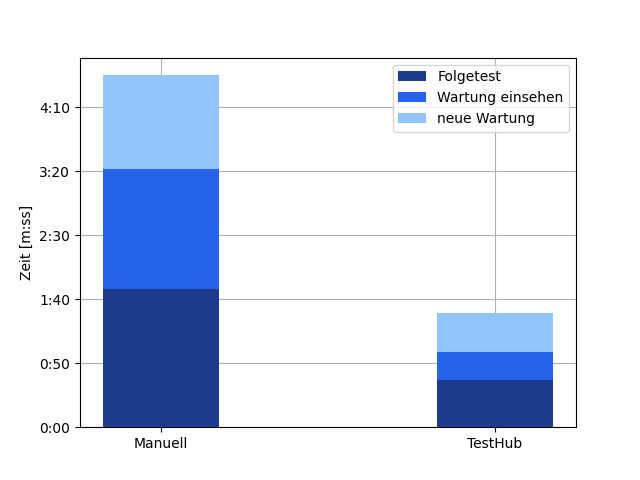
\includegraphics[width=\linewidth]{speedtests/validierung_Zeit.png}
      \caption{Zeitersparnis}
    \end{subfigure}%
    \begin{subfigure}{.5\textwidth}
      \centering
      \includegraphics[width=\linewidth]{speedtests/validierung_cursordistanz.png}
      \caption{Mauszeigerdistanz}
    \end{subfigure}\\
    \begin{subfigure}{.5\textwidth}
        \centering
        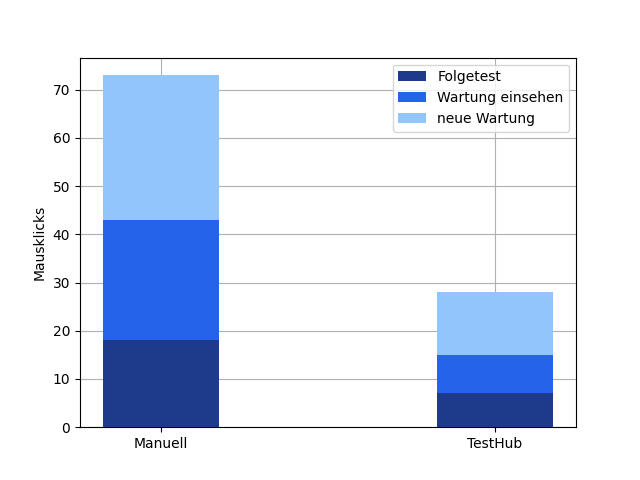
\includegraphics[width=\linewidth]{speedtests/validierung_Mausklicks.png}
        \caption{Mausklicks}
      \end{subfigure}%
      \begin{subfigure}{.5\textwidth}
        \centering
        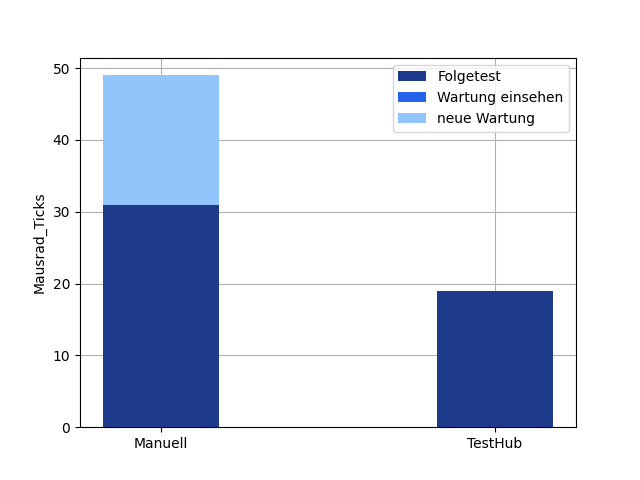
\includegraphics[width=\linewidth]{speedtests/validierung_Mausrad_Ticks.png}
        \caption{Mausrad Ticks}
      \end{subfigure}
    \caption{Ergebnisse der Bedienbarkeitsvalidierung, aufgeschlüsselt nach Aufgaben}
   
\end{figure}

\begin{longtable}{| P{0.15\linewidth} | P{0.15\linewidth} | P{0.15\linewidth} | P{0.15\linewidth} | P{0.15\linewidth} |} 
  \hline
  \textbf{Aufgabe} & \textbf{Zeit} & \textbf{Mauszeiger- distanz} & \textbf{Klickzahl} & \textbf{Mausrad Ticks}\\[0.5ex] 
  \hline
  
  Folgeticket & 65,74\% & 70,13\% & 61,11\% & 38,71\% \\ [0.5ex] \hline
  Wartung einsehen & 76,60\% & 66,68\% & 68,00\% & - \\ [0.5ex] \hline
  neuer Wartungstermin & 58,91\% & -12,46\% & 56,67\% & 100\% \\ [0.5ex] \hline
  \textbf{Gesamt} & 67,64\% & 45,59\% & 61,64\% & 61,22\% \\ [0.5ex] \hline
  \caption{Verbesserung des alten Prozesses durch TestHub nach Aufgaben aufgeschlüsselt }\label{tab:valres}
\end{longtable}

\textit{Tests wurden lokal auf einem Dell Latitude 5590 (Intel Core i5-8350U CPU
@ 1.70GHz; 8GB RAM) mit angeschlossenem 32'' Bildschirm mit 4K (3840$\times$2160) Auflösung im HomeOffice durchgeführt} \\[2ex]



Auf den ersten subjektiven Blick fällt auf, dass TestHub in fast allen Bereichen eine erhebliche
Verbesserung aufweist. Gerade der wichtigste Faktor, der Zeitaufwand, ist durch TestHub 
mit einer Verbesserung von ca. 70\% erheblich geringer. Nur bei der Erstellung eines neuen Wartungstermins
ist die Mauszeigerdistanz etwas größer als bisher, da in einem maximierten Browserfenster
gearbeitet wird statt im kleinen Windows Dateiexplorer Fenster. Da jedoch der 
Zeitaufwand trotzdem geringer ist, fällt dies nicht ins Gewicht.
Auch auffallend ist,
dass nur beim Folgetest heraussuchen das Mausrad benutzt werden muss. Die Benutzung des 
Mausrads beim Erstellen eines neuen Wartungstermins fällt komplett weg, was für 
eine Übersichtlichkeit des Projekts spricht.

Um diese Aussagen zu belegen, müsste jedoch eine viel größere Studie mit mehreren 
Teilnehmern und Testfällen durchgeführt werden.

\newpage




\section{Fazit}

Das im Rahmen dieser Arbeit entwickelte Programm ``TestHub'' konnte erfolgreich 
als \gls{MVP} umgesetzt werden. Fast alle der zuvor definierten Anforderungen wurden
erfüllt. Somit wurden auch die zu Beginn angesprochenen Probleme, wie etwa der 
komplizierte Prozess zum Einsehen eines Wartungstermins, verbessert und gelöst werden.
Dazu wurde ein Joyson Safety Systems spezifisches Programm entwickelt, welches
genau auf das teilweise stark individualisierte Jira-Ticket-System angepasst wurde. 
Nicht nur Jira Informationen wurden in TestHub eingebunden, sondern es wurde auch 
eine zentrale und universelle einsetzbare Anlaufstelle für jegliche weitere 
Ressourcen geschaffen. Durch TestHub sind alle Ressourceninformationen, welche
man für benötigt, um einen Test aufzubauen und durchzuführen, an der gleichen Stelle 
und lassen sich schnell und effizient einsehen und bearbeiten. Das in der 
Client-Server Architektur entwickelte System erleichtert heute schon vielen Mitarbeitern
die Arbeit. TestHub stellt außerdem eine \gls{REST} \gls{API} innerhalb der Firma 
zur Verfügung, wodurch andere Programme die von TestHub verwendeten und verarbeiteten 
Informationen verwerten können. Durch die Verwendung von modernen und aufstrebenden Technologien,
wie Typescript oder der Programmiersprache Go, ist das Programm erweiterbar 
und zukunftssicher.\\

Jedoch gibt es bei \gls{JSS} nur wenige Entwickler, welche diese Sprachen beherrschen.
Allerdings werden auch keine komplexen sprachenspezifischen Konzepte genutzt, wodurch
der Einstieg in die Entwicklung dieses Projekts erleichtert wird. Zu diesem Zweck
wurde auch eine \textit{setup.md} erstellt, welche Entwicklern beim Start der
Entwicklung dieses Projekts helfen soll. Zusätzlich ist der Code umfangreich kommentiert.

\subsection{Ausblick}
Um die gesteigerte Effizienz auch wirklich belegen zu können sollten aussagekräftige
Studien zur Bedienbarkeit und Benutzung von TestHub durchgeführt werden.
Die nicht erfüllten Anforderungen geben einen kurzen Überblick über Möglichkeiten
das Projekt weiterzuführen. Besonders das Gantt-Diagramm würde eine gute Ergänzung
zur Übersichtlichkeit und Nachvollziehbarkeit der Teststruktur liefern und dafür
wäre auch noch genug Platz auf dem Dashboard.
Eine weitere Überlegung ist es, Benutzeraccounts einzuführen. Da bei einer Wartung
die Wartende Person manuell eingetragen wird, lässt dies Platz für Falscheingaben und Fehler. 
Durch die Einbindung von Benutzeraccounts kann man eher gewährleisten, dass die 
wartende Person auch tatsächlich die eingetragene Person ist. Dafür könnte OAuth
von Microsoft oder Jira verwendet werden. OAuth bietet dabei die Möglichkeit, dass
die Verwaltung der Benutzerdaten nicht von TestHub übernommen werden muss. TestHub
wird lediglich als Programm registriert und leitet den Benutzer weiter, sodass er sich
bei dem entsprechendem Service anmeldet. Anschließend erhält TestHub die Accountdaten
des Nutzers. Beide dieser OAuth Möglichkeiten sind aber noch nicht für eigens entwickelte 
Anwendungen innerhalb der Firma nutzbar.

\begin{spacing}{1}
    \pagenumbering{Roman}
    \setcounter{page}{7}

    \section*{Literaturverzeichnis}
    \addcontentsline{toc}{section}{Literaturverzeichnis}
    \printbibliography[title={Fachliteratur},type=book]
    \printbibliography[title={Onlinequellen},type=online]
    \newpage
    \begin{spacing}{1}
            
        \section*{Abbildungsverzeichnis} 
        \addcontentsline{toc}{section}{Abbildungsverzeichnis}
        \renewcommand{\listfigurename}{}
        \listoffigures
    \end{spacing}
    \newpage

    \section*{Tabellenverzeichnis} 
    \addcontentsline{toc}{section}{Tabellenverzeichnis} 
    \renewcommand{\listtablename}{}
    \listoftables % Tabellenverzeichnis
    \newpage

    \addcontentsline{toc}{section}{Codebeispielverzeichnis} 
    \lstlistoflistings


    
\section*{Anhang}\label{sec:anhang}
\addcontentsline{toc}{section}{Anhang} 

\appendix
\section*{A. Allgemeine Ergänzungen}
Dieser Arbeit wurde ein USB-Stick beigelegt, welcher den gesamten im Rahmen 
dieser Arbeit verfassten Quellcode und das zuvor angeführte Video enthält. Die
Ordnerstruktur ist wie folgt angelegt:

\begin{description}
    \item[\textit{./backend}] $\rightarrow$~die serverseitige Software (Go)

    \item[\textit{./data}] $\rightarrow$~Daten auf die der Server zur Laufzeit 
    zugreifen muss

    \item[\textit{./frontend}] $\rightarrow$~die clientseitige Software 
    (\textit{./frontend/ts}) und der Stylesheet (\textit{./frontend/css})

    \item[\textit{./static}] $\rightarrow$~statische Dateien wie Bilder oder Vektorgrafiken.
    Außerdem werden die von TypeScript kompilierten JavaScript Dateien und der 
    von TailwindCSS generierte Stylesheet hier abgelegt.

    \item[\textit{./templates}] $\rightarrow$~Die HTML Templates welche vom Server
    zu einem richtigen HTML Dokument zusammengesetzt werden.
    
    \item[\textit{./videos}] $\rightarrow$~Das zuvor angeführte Video.

\end{description}

\section*{B. Webservertest Quellcode}
\lstinputlisting[language=Python, caption=Python Flask Webserver]{resources/python.py}

\lstinputlisting[language=Go, caption=Go Webserver]{resources/go.go}

\lstinputlisting[language=Python, caption=Python Testskript]{resources/test.py}

\section*{C. Tagesplan und Ressourcenliste}
\begin{figure}[H]
    \includegraphics[width=\linewidth]{img/tagesplan_auszug_02_03_22.png}
    \caption{Auszug eines Tagesplans vom 02.03.2022}\label{fig:tagesplan}
\end{figure}

\begin{figure}[H]
    \includegraphics[width=\linewidth]{img/ressourcenliste_auszug_26_03_22.png}
    \caption{Übersichtsseite der Ressourcenliste vom 26.03.2022}\label{fig:ressourcenliste}
\end{figure}
\end{spacing}
\end{document}